\chapter{Numerical Analysis: Results of Simulations}


\section{First usage of the Adaptive Algorithm}


\willdo{changer le nom du 10. et suivants.}
\begin{figure}
\centering
\subfloat{{
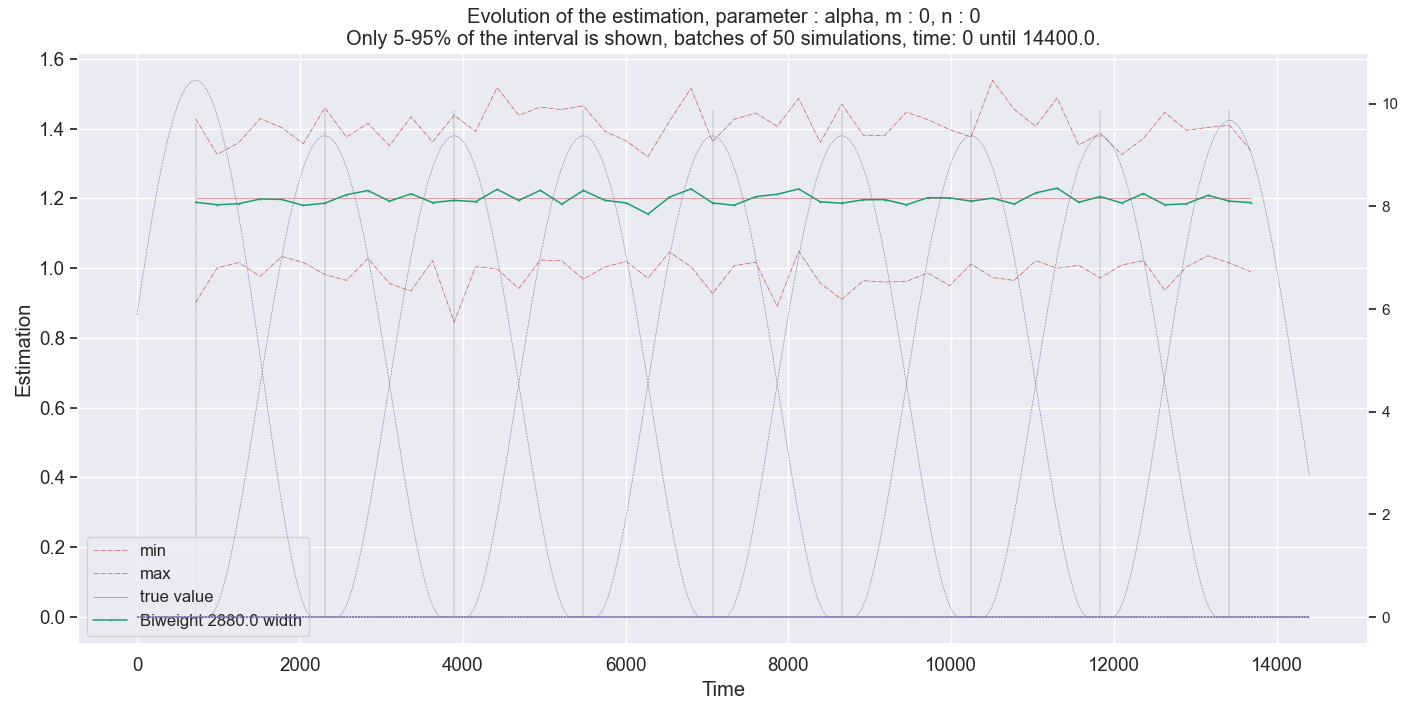
\includegraphics[width = 0.48 \textwidth]{../imag/chap3/0/Figure_2.png}
}} 
\subfloat{{
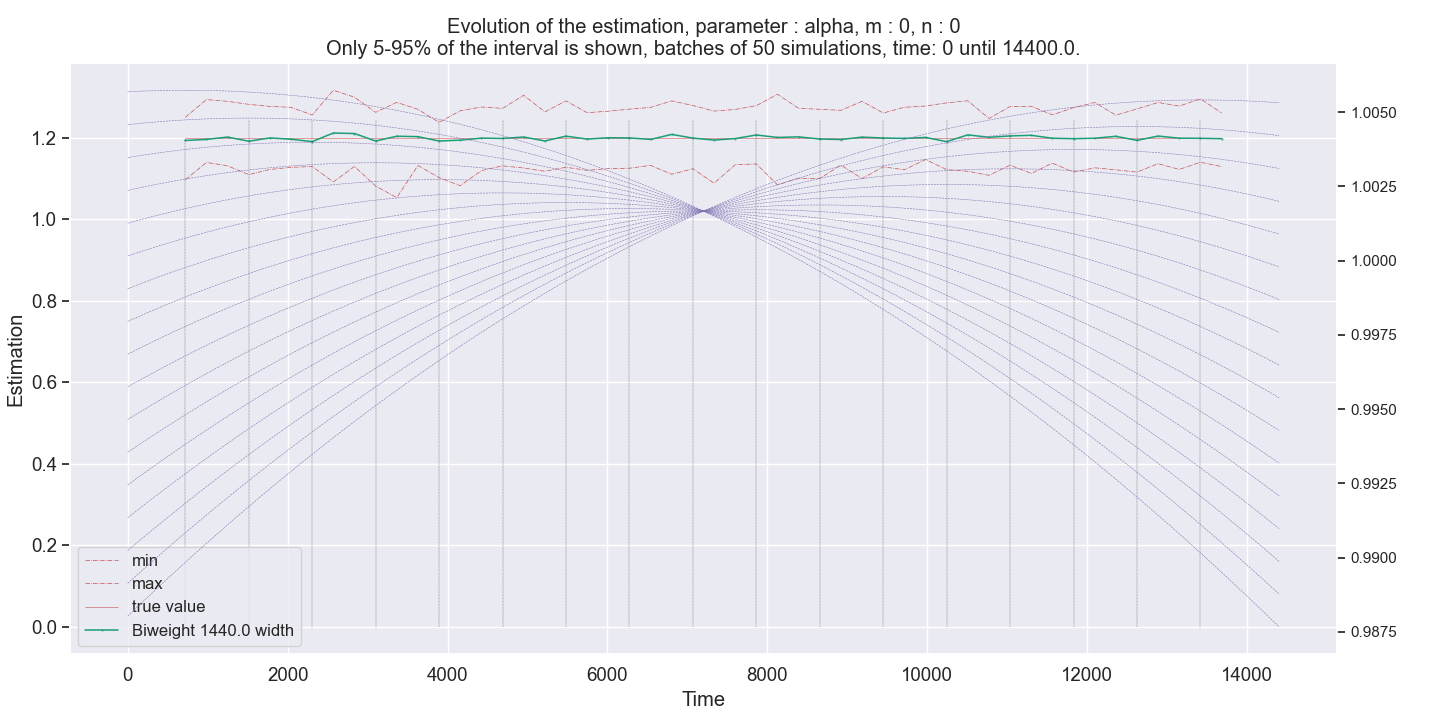
\includegraphics[width = 0.48 \textwidth]{../imag/chap3/0/Figure_10.png}
}}
\caption{We observe how the first kernels evolved into the second set of kernels in the case of constant parameters.}
\label{fig:compar_kernels_0}
\end{figure}


\begin{figure}
\centering
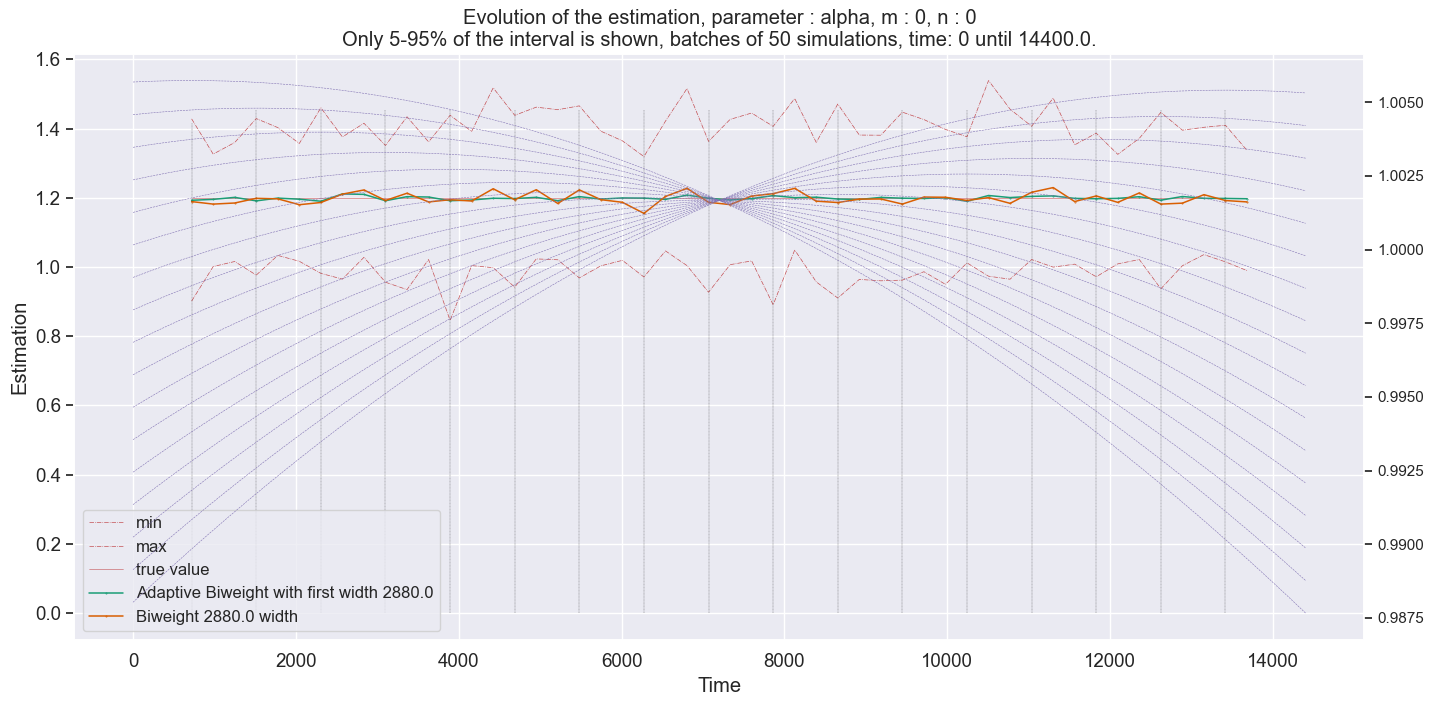
\includegraphics[width = 0.90 \textwidth]{../imag/chap3/0/A.png}
\caption{TO WRITE.}
\label{fig:first_estimate_0_alpha}
\end{figure}

\begin{figure}
\centering
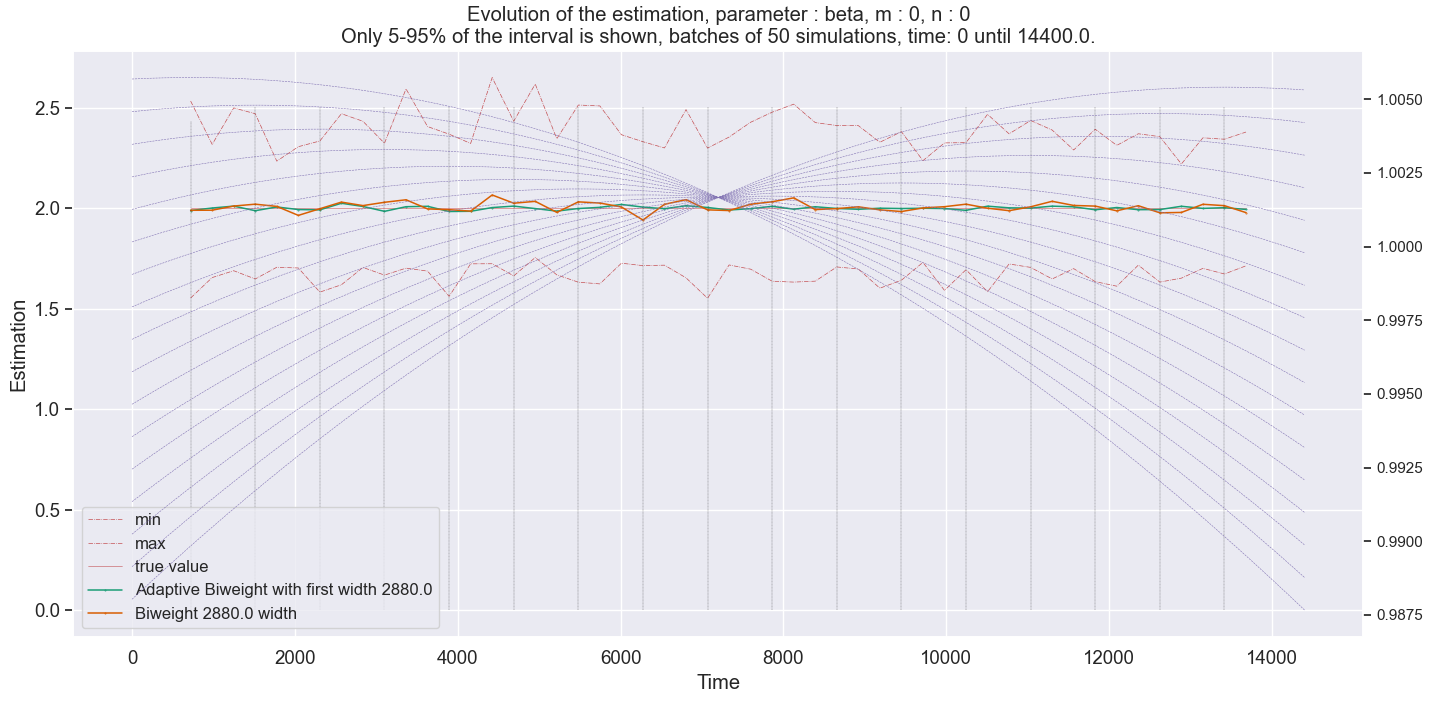
\includegraphics[width = 0.90 \textwidth]{../imag/chap3/0/B.png}
\caption{TO WRITE.}
\label{fig:first_estimate_0_beta}
\end{figure}

\begin{figure}
\centering
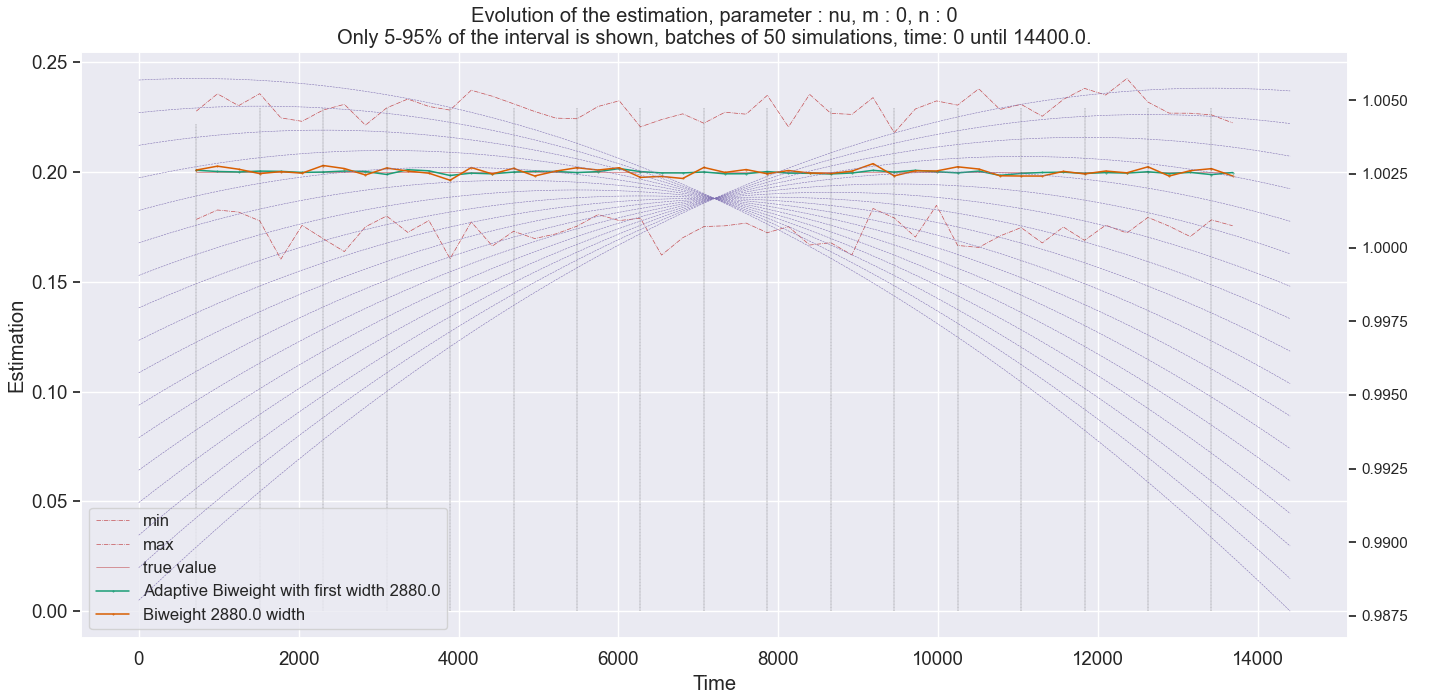
\includegraphics[width = 0.90 \textwidth]{../imag/chap3/0/C.png}
\caption{TO WRITE.}
\label{fig:first_estimate_0_nu}
\end{figure}











\willdo{le nom...}
\begin{figure}
\centering
\subfloat{{
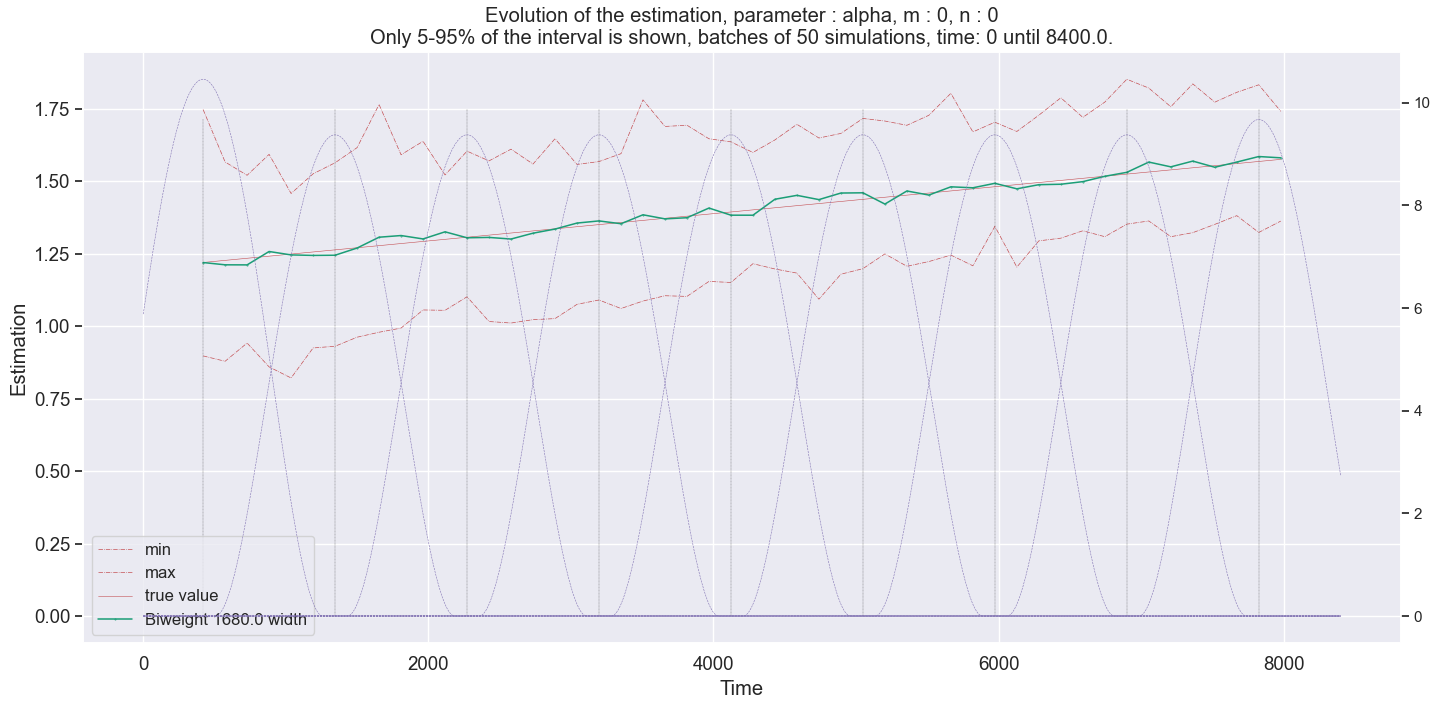
\includegraphics[width = 0.48 \textwidth]{../imag/chap3/1/Figure_2.png}
}} 
\subfloat{{
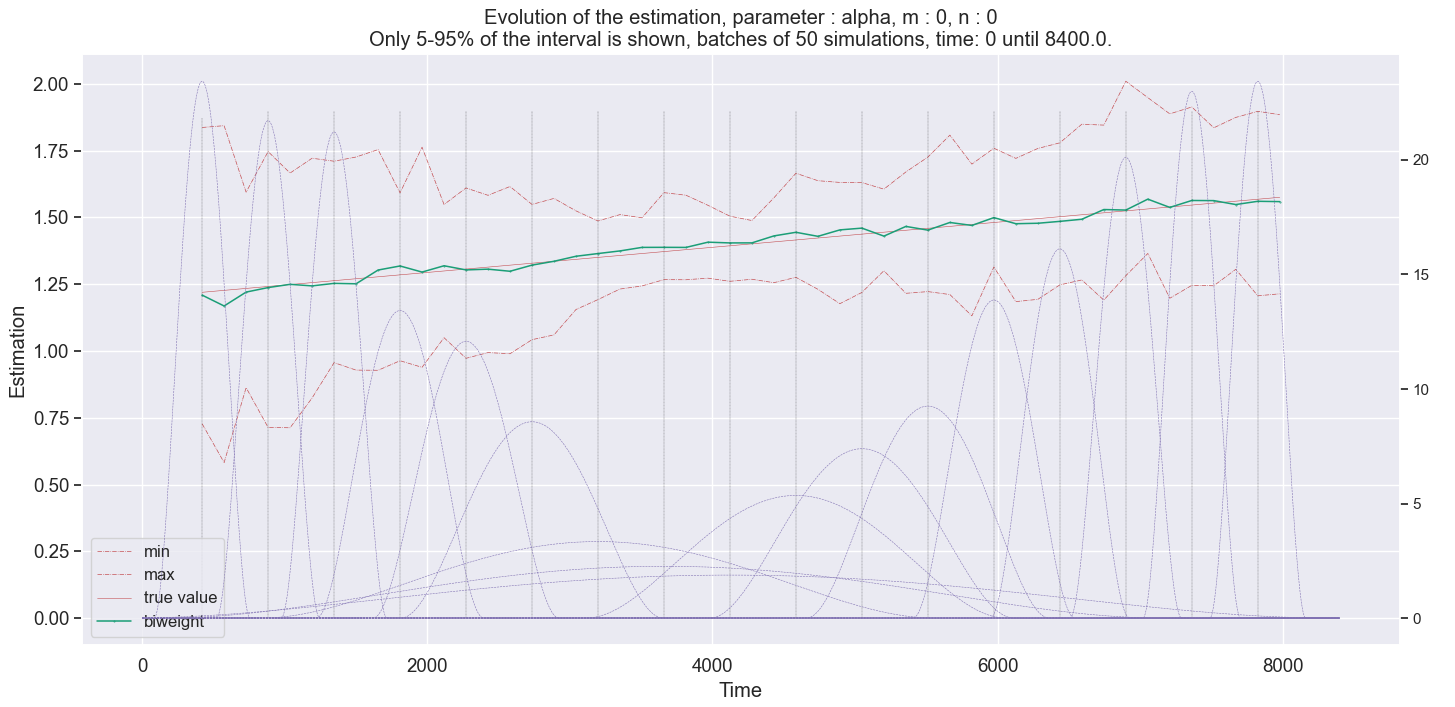
\includegraphics[width = 0.48 \textwidth]{../imag/chap3/1/Figure_10.png}
}}
\caption{We observe how the first kernels evolved into the second set of kernels in the case of linear growth.}
\label{fig:compar_kernels_1}
\end{figure}

\begin{figure}
\centering
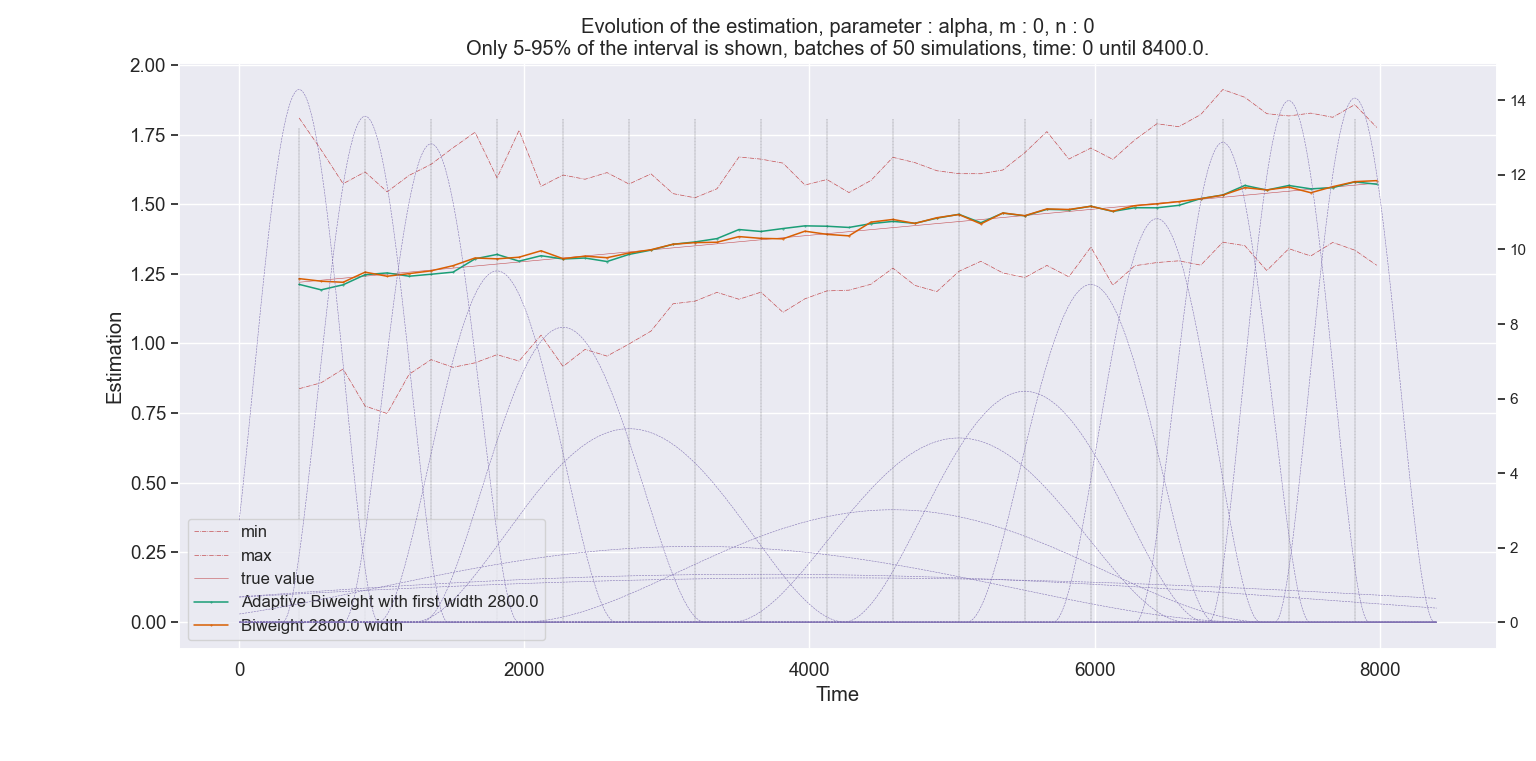
\includegraphics[width = 0.90 \textwidth]{../imag/chap3/1/D.png}
\caption{TO WRITE.}
\label{fig:first_estimate_1_alpha}
\end{figure}

\begin{figure}
\centering
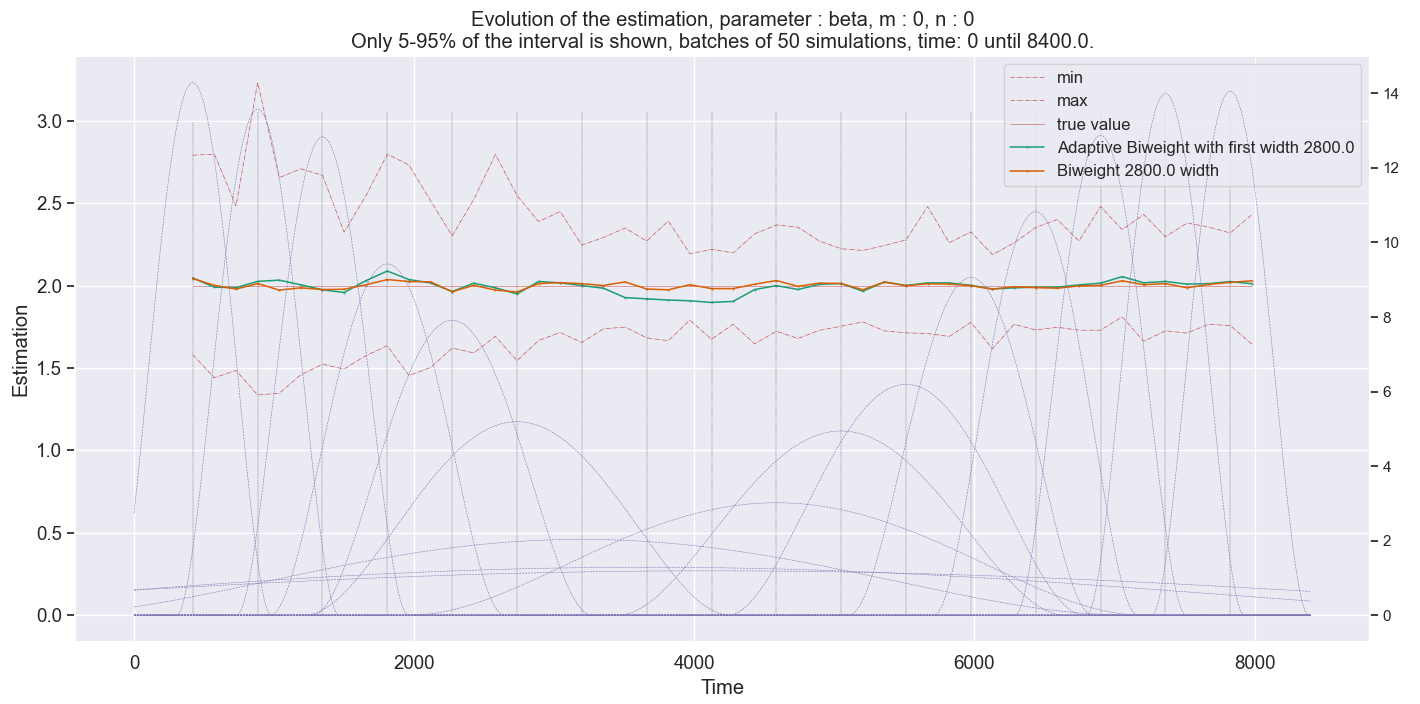
\includegraphics[width = 0.90 \textwidth]{../imag/chap3/1/E.png}
\caption{TO WRITE.}
\label{fig:first_estimate_1_beta}
\end{figure}

\begin{figure}
\centering
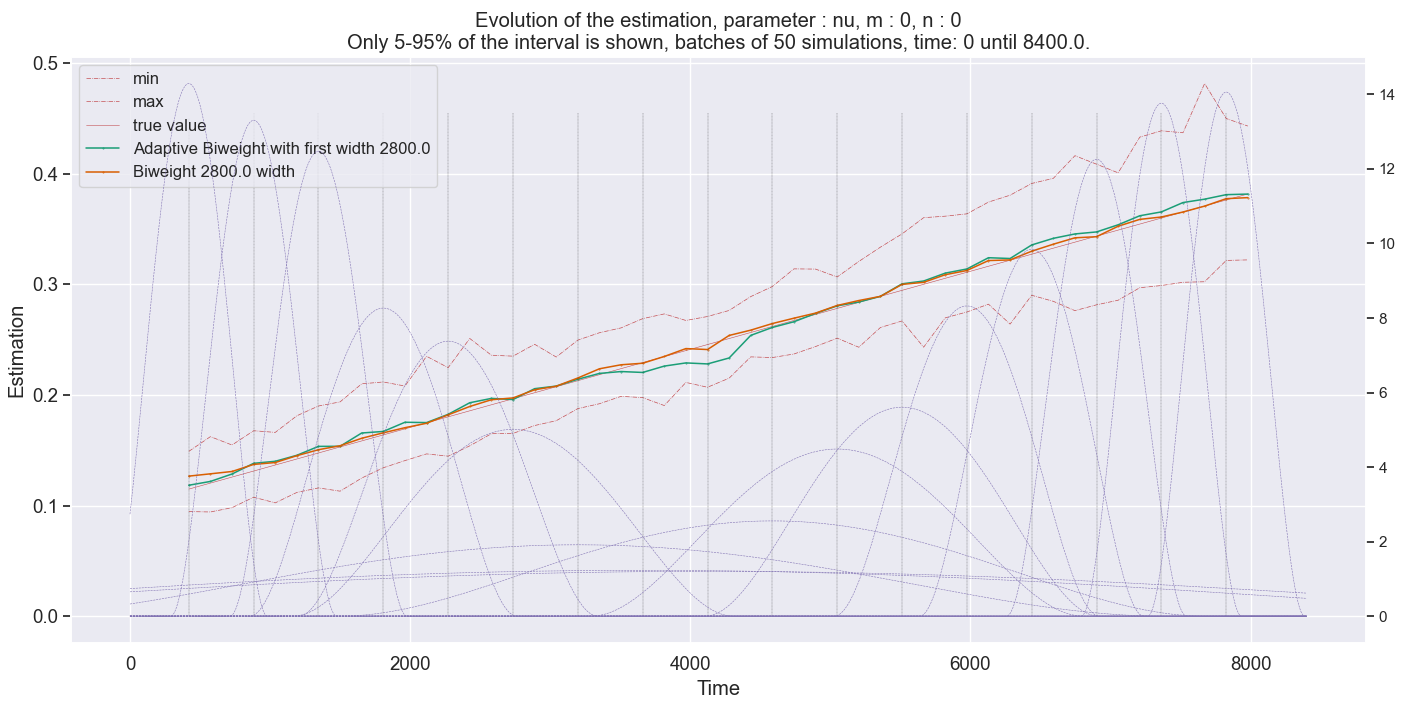
\includegraphics[width = 0.90 \textwidth]{../imag/chap3/1/F.png}
\caption{TO WRITE.}
\label{fig:first_estimate_1_nu}
\end{figure}

















\begin{figure}
\centering
\subfloat{{
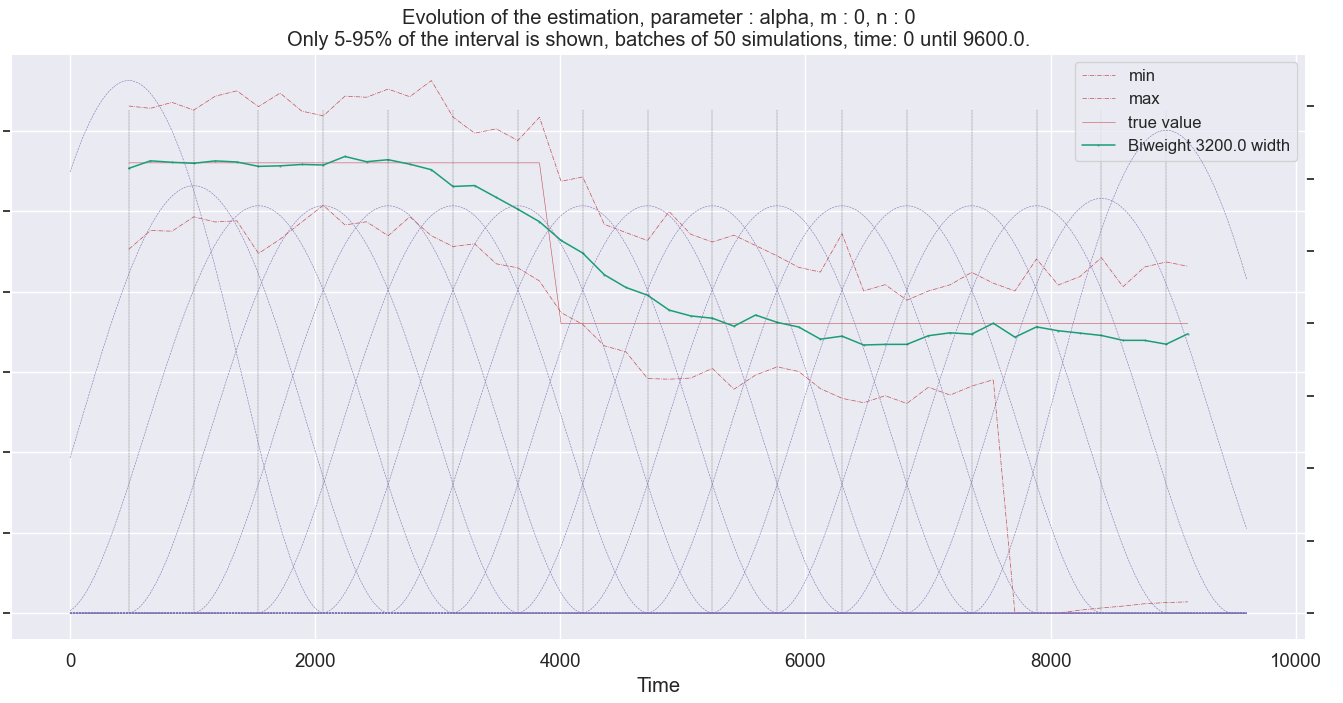
\includegraphics[width = 0.48 \textwidth]{../imag/chap3/2/Figure_2.png}
}} 
\subfloat{{
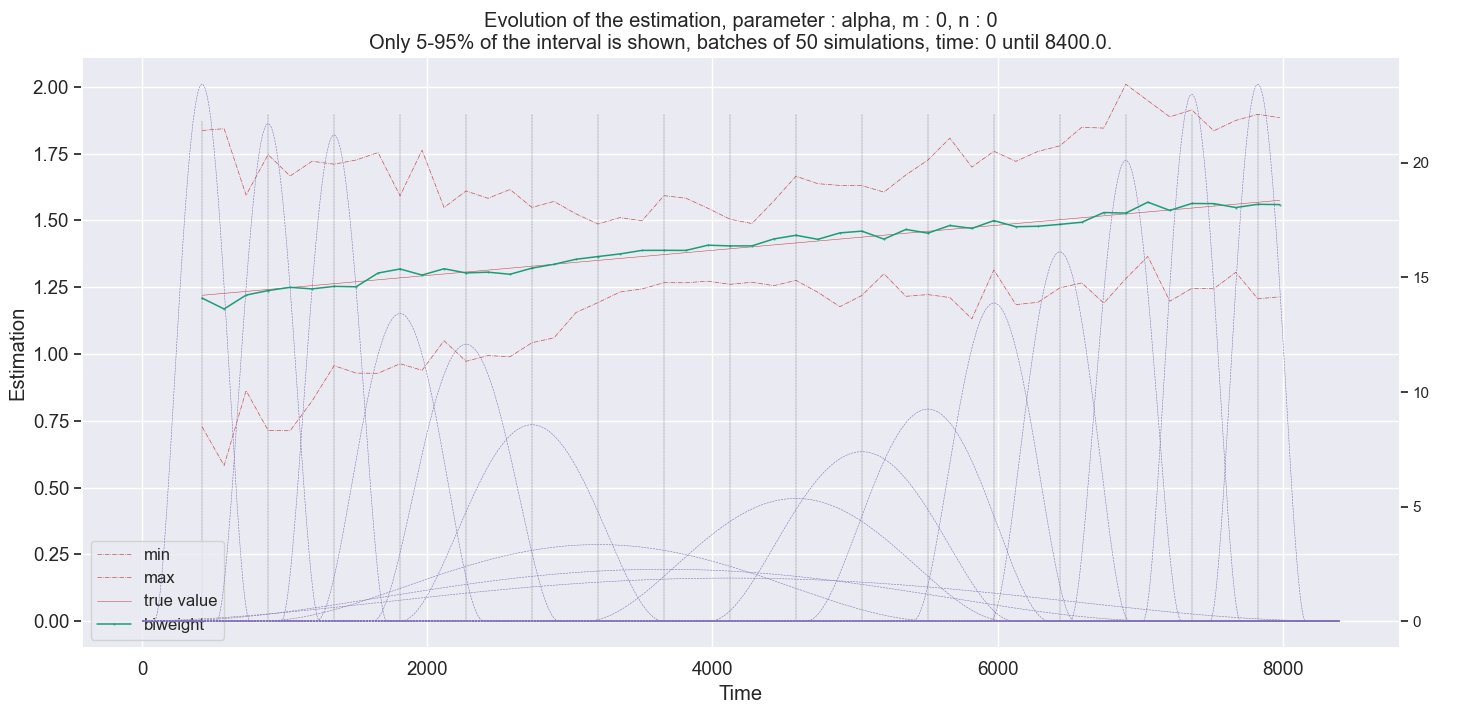
\includegraphics[width = 0.48 \textwidth]{../imag/chap3/2/Figure_10.png}
}}
\caption{We observe how the first kernels evolved into the second set of kernels in the case of a jump evolving parameters.}
\label{fig:compar_kernels_2}
\end{figure}

\begin{figure}
\centering
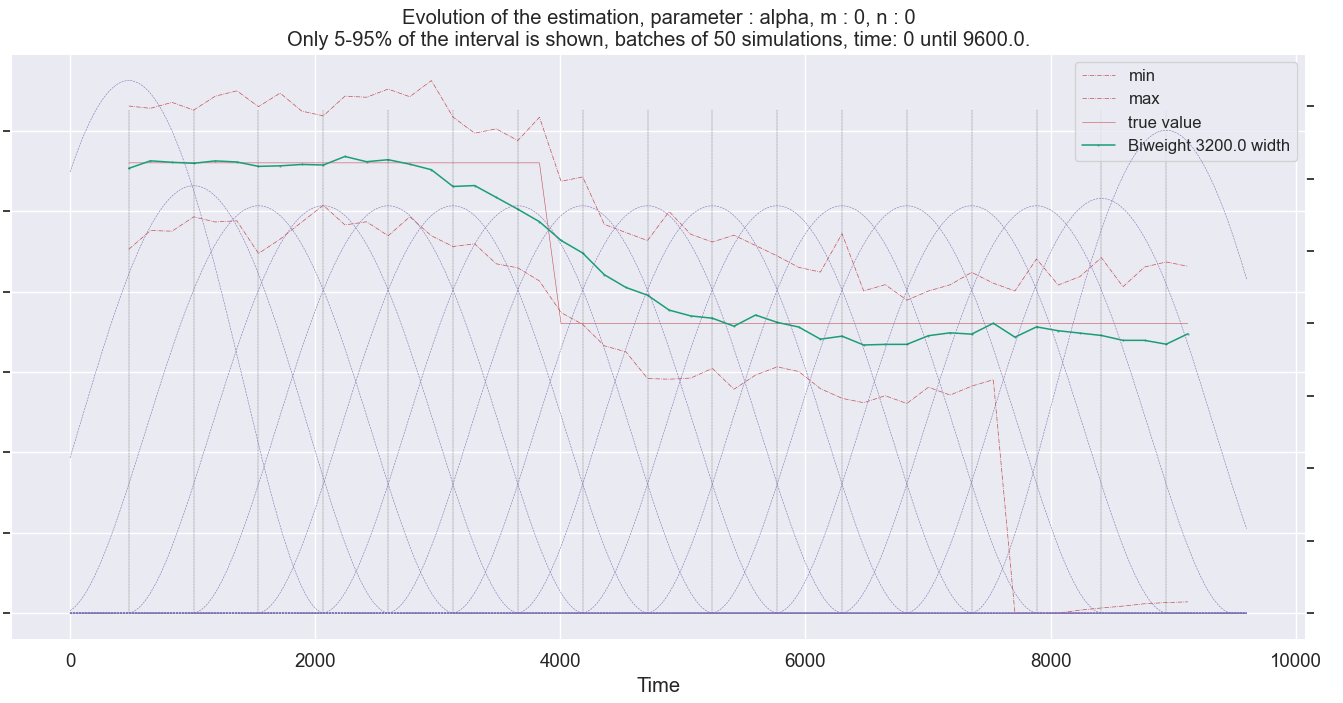
\includegraphics[width = 0.90 \textwidth]{../imag/chap3/2/Figure_2.png}
\caption{TO WRITE.}
\label{fig:first_estimate_2_alpha}
\end{figure}

\begin{figure}
\centering
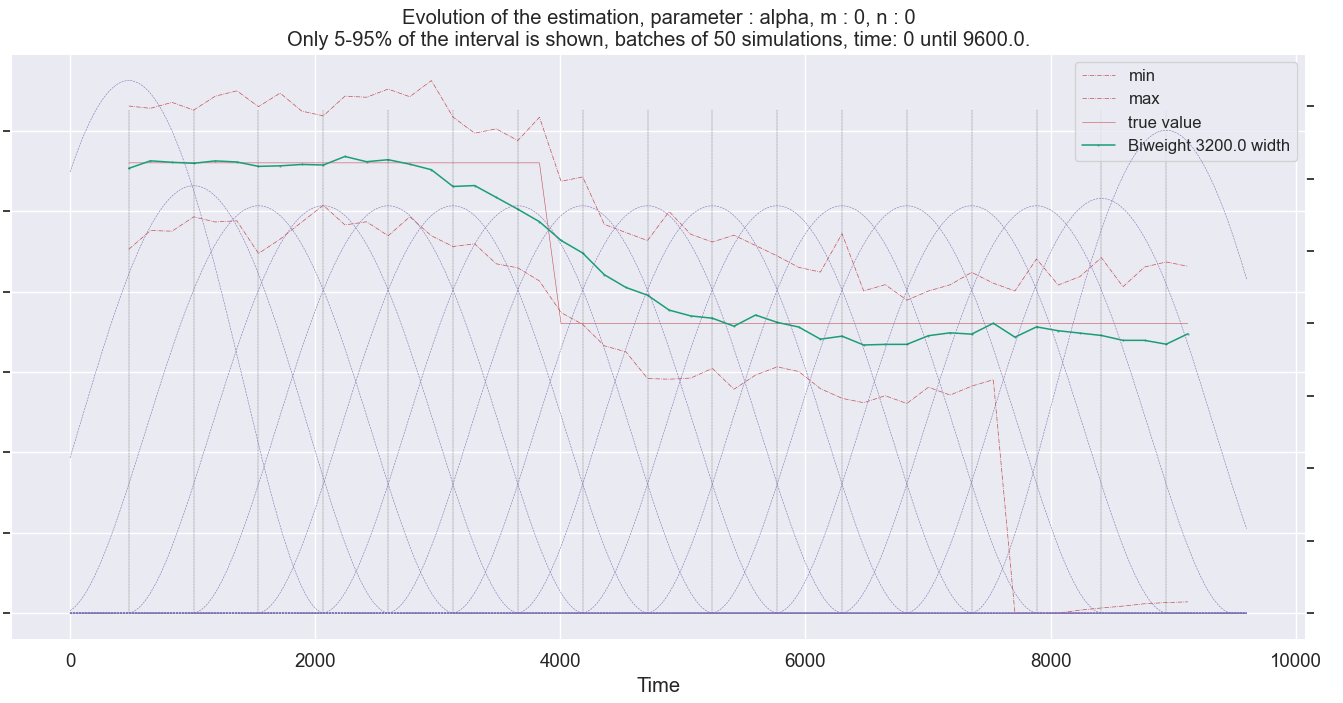
\includegraphics[width = 0.90 \textwidth]{../imag/chap3/2/Figure_2.png}
\caption{TO WRITE.}
\label{fig:first_estimate_2_beta}
\end{figure}

\begin{figure}
\centering
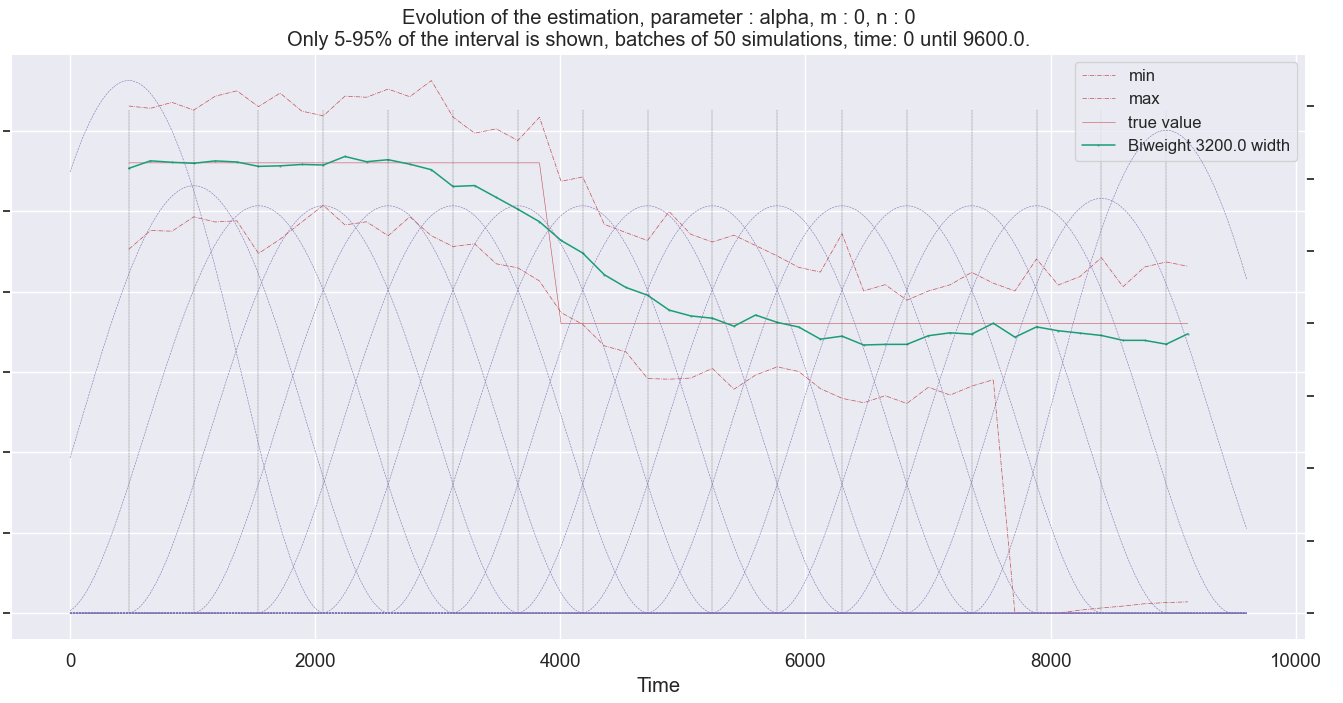
\includegraphics[width = 0.90 \textwidth]{../imag/chap3/2/Figure_2.png}
\caption{TO WRITE.}
\label{fig:first_estimate_2_nu}
\end{figure}



















\begin{figure}
\centering
\subfloat{{
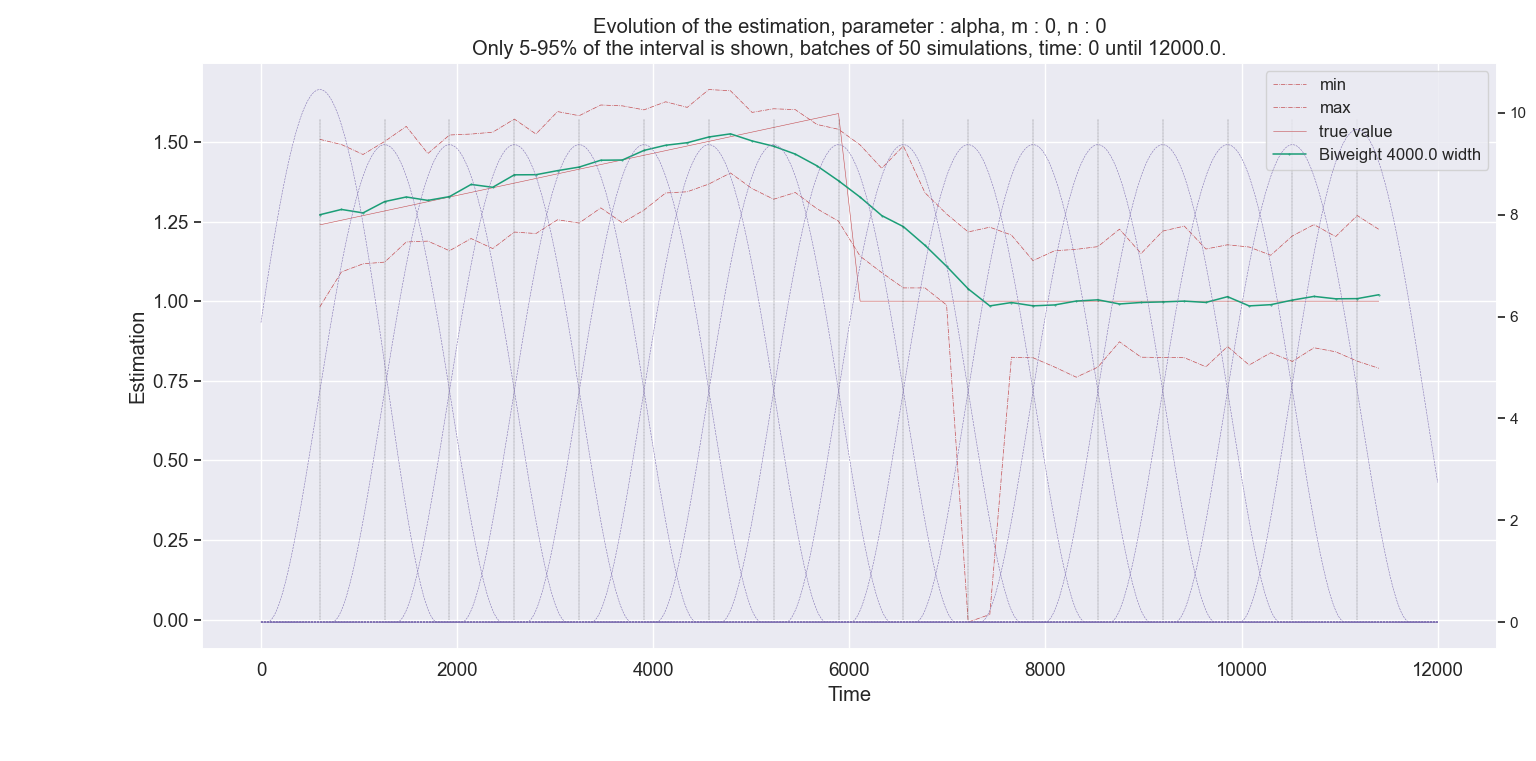
\includegraphics[width = 0.48 \textwidth]{../imag/chap3/3/Figure_2.png}
}} 
\subfloat{{
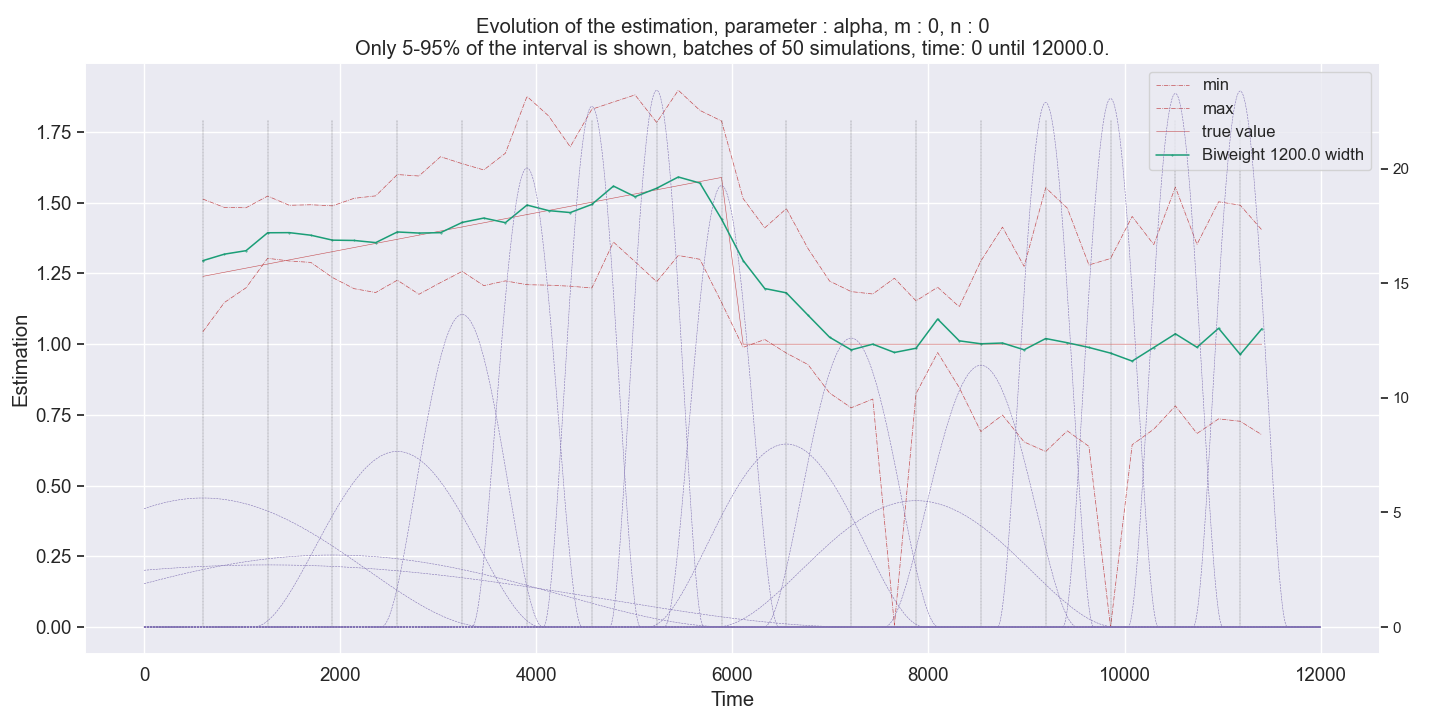
\includegraphics[width = 0.48 \textwidth]{../imag/chap3/3/Figure_10.png}
}}
\caption{We observe how the first kernels evolved into the second set of kernels in the jump and linear growth case.}
\label{fig:compar_kernels_3}
\end{figure}

\begin{figure}
\centering
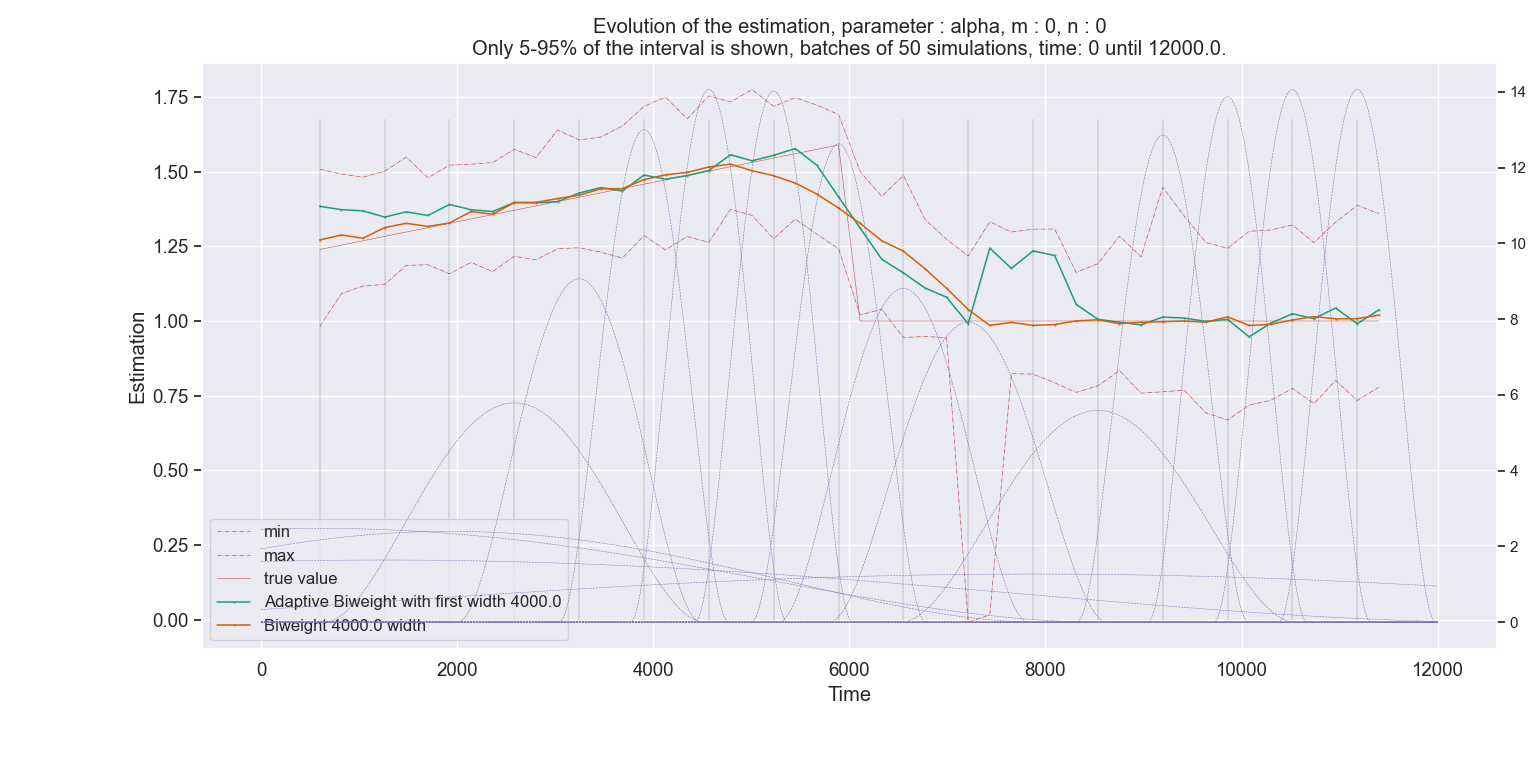
\includegraphics[width = 0.90 \textwidth]{../imag/chap3/3/J.png}
\caption{TO WRITE.}
\label{fig:first_estimate_3_alpha}
\end{figure}

\begin{figure}
\centering
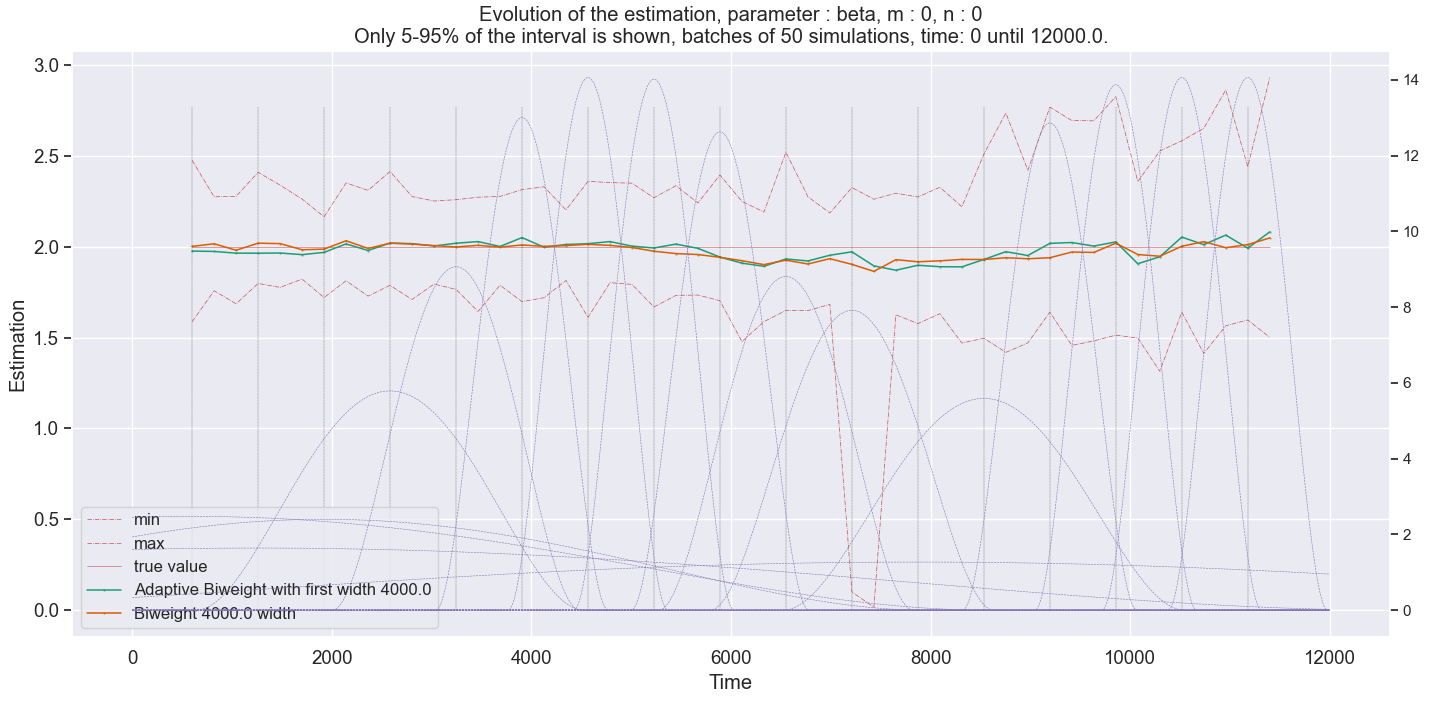
\includegraphics[width = 0.90 \textwidth]{../imag/chap3/3/K.png}
\caption{TO WRITE.}
\label{fig:first_estimate_3_beta}
\end{figure}

\begin{figure}
\centering
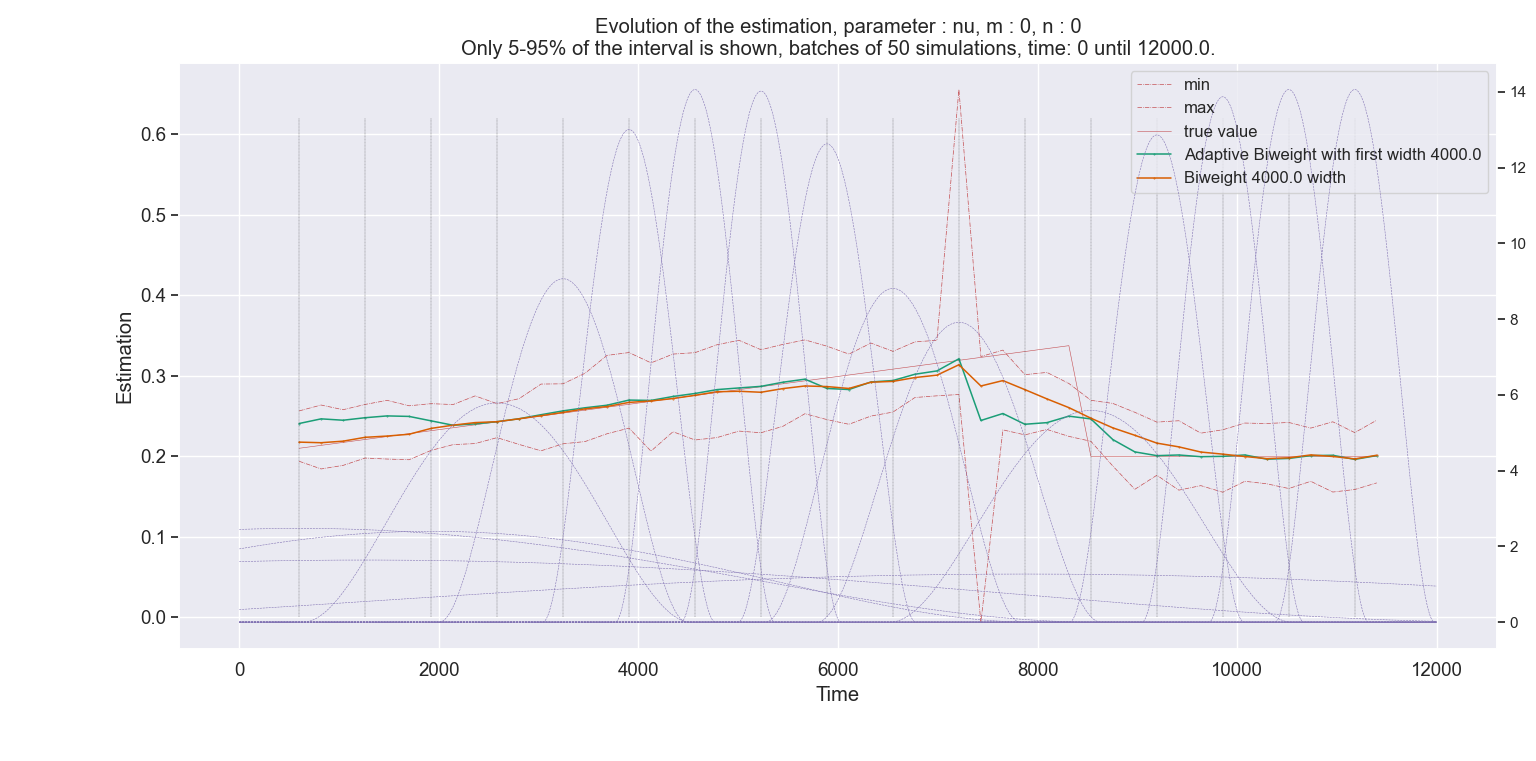
\includegraphics[width = 0.90 \textwidth]{../imag/chap3/3/L.png}
\caption{TO WRITE.}
\label{fig:first_estimate_3_nu}
\end{figure}















\begin{figure}
\centering
\subfloat{{
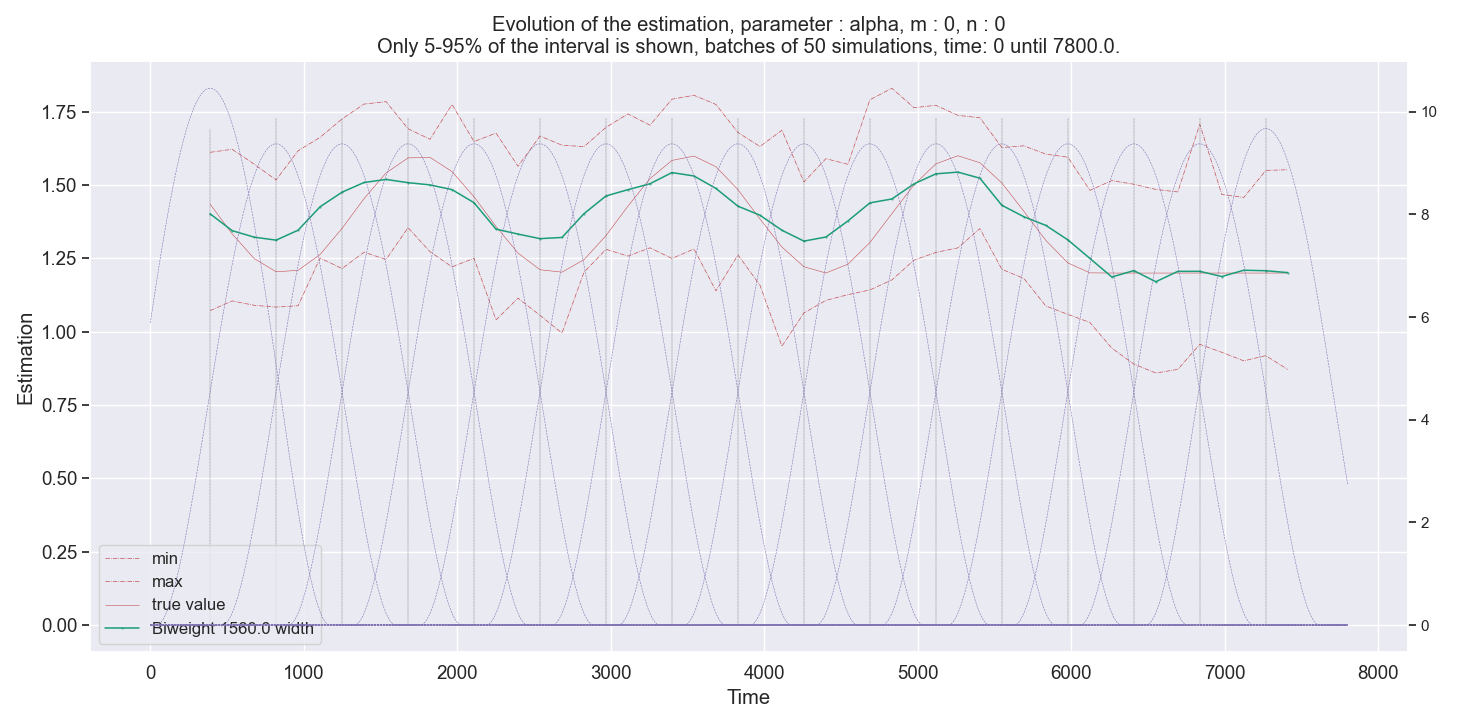
\includegraphics[width = 0.48 \textwidth]{../imag/chap3/4/Figure_2.png}
}} 
\subfloat{{
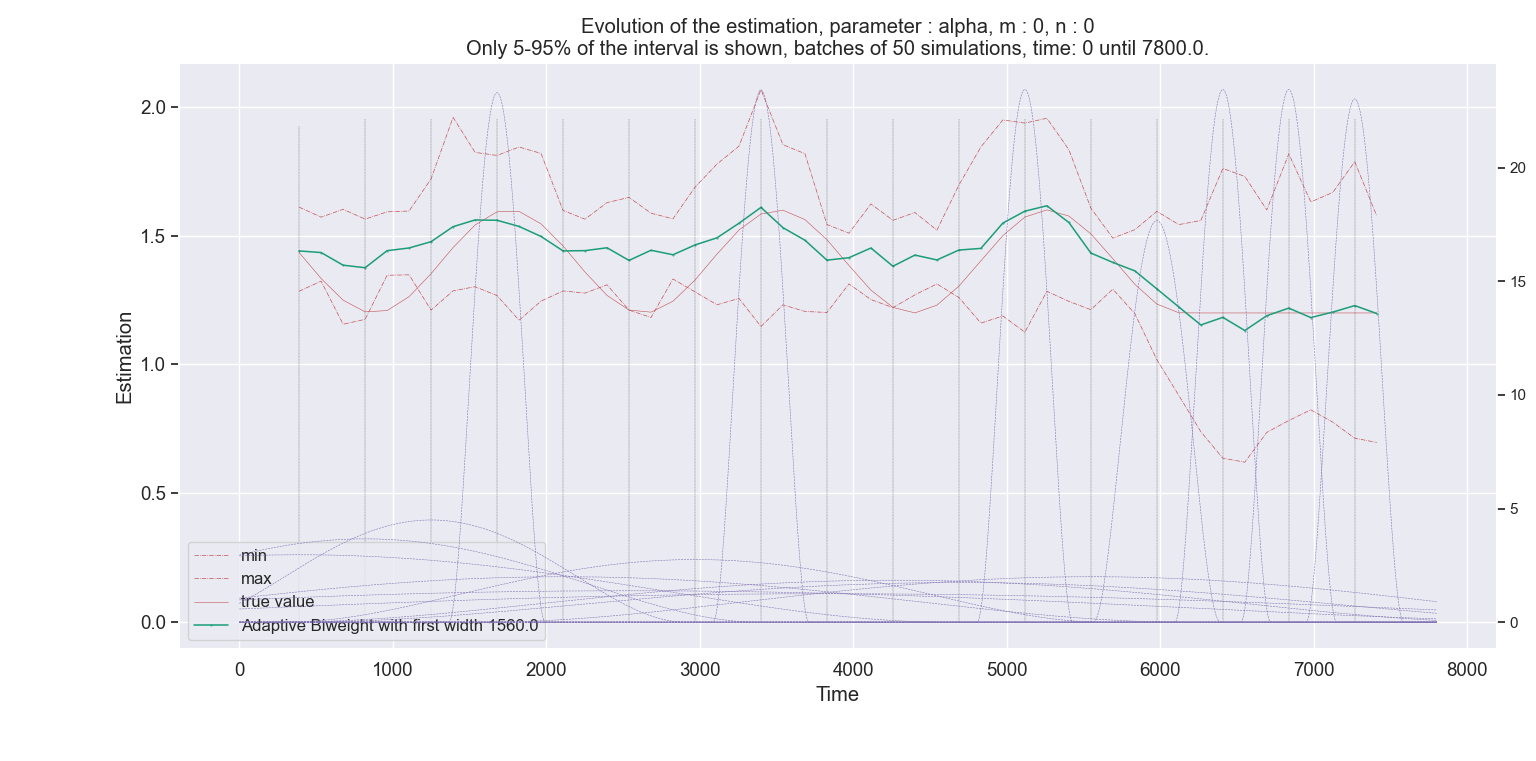
\includegraphics[width = 0.48 \textwidth]{../imag/chap3/4/Figure_10.png}
}}
\caption{We observe how the first kernels evolved into the second set of kernels in the sinus case.}
\label{fig:compar_kernels_4}
\end{figure}

\begin{figure}
\centering
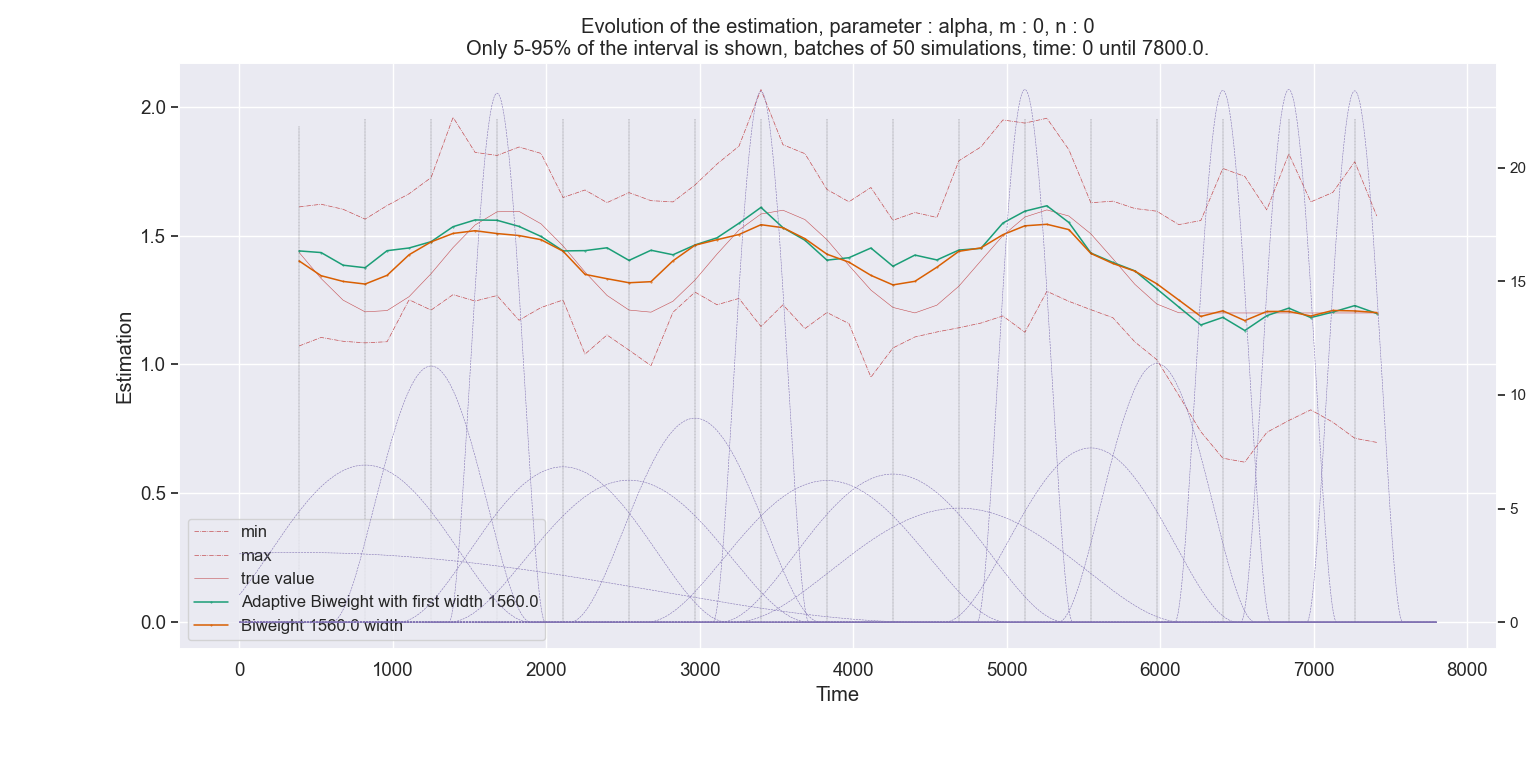
\includegraphics[width = 0.90 \textwidth]{../imag/chap3/4/M.png}
\caption{TO WRITE.}
\label{fig:first_estimate_4_alpha}
\end{figure}

\begin{figure}
\centering
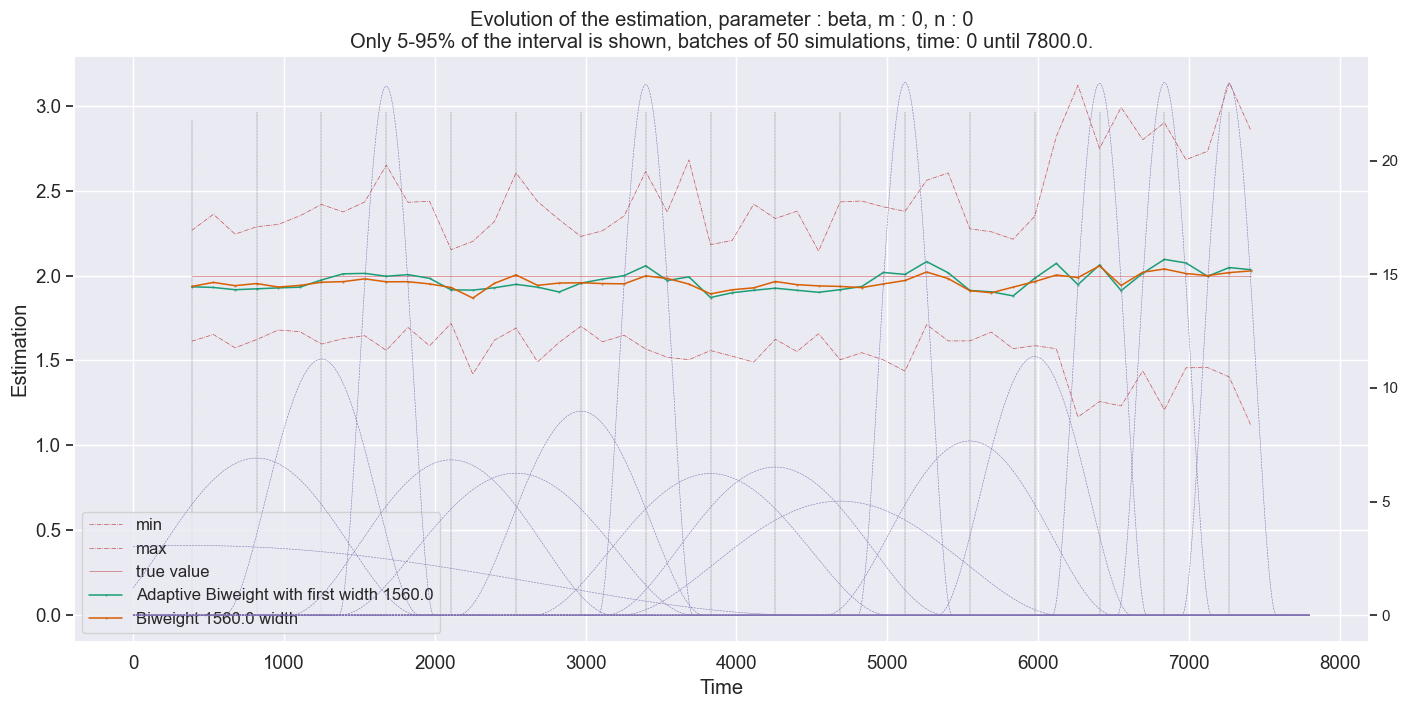
\includegraphics[width = 0.90 \textwidth]{../imag/chap3/4/N.png}
\caption{TO WRITE.}
\label{fig:first_estimate_4_beta}
\end{figure}

\begin{figure}
\centering
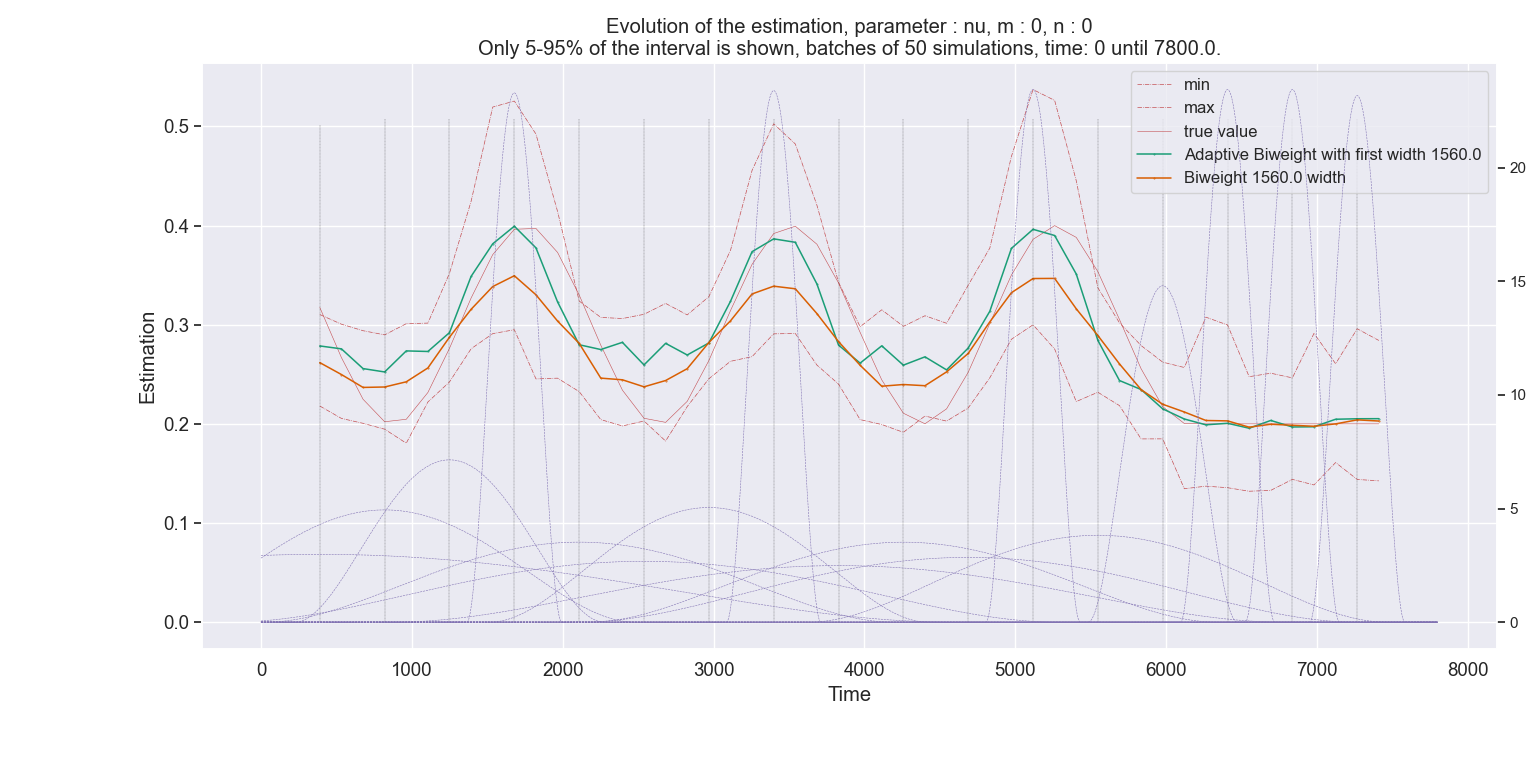
\includegraphics[width = 0.90 \textwidth]{../imag/chap3/4/O.png}
\caption{TO WRITE.}
\label{fig:first_estimate_4_nu}
\end{figure}






































\newpage
\section{Better First Guess}



\begin{figure}
\centering
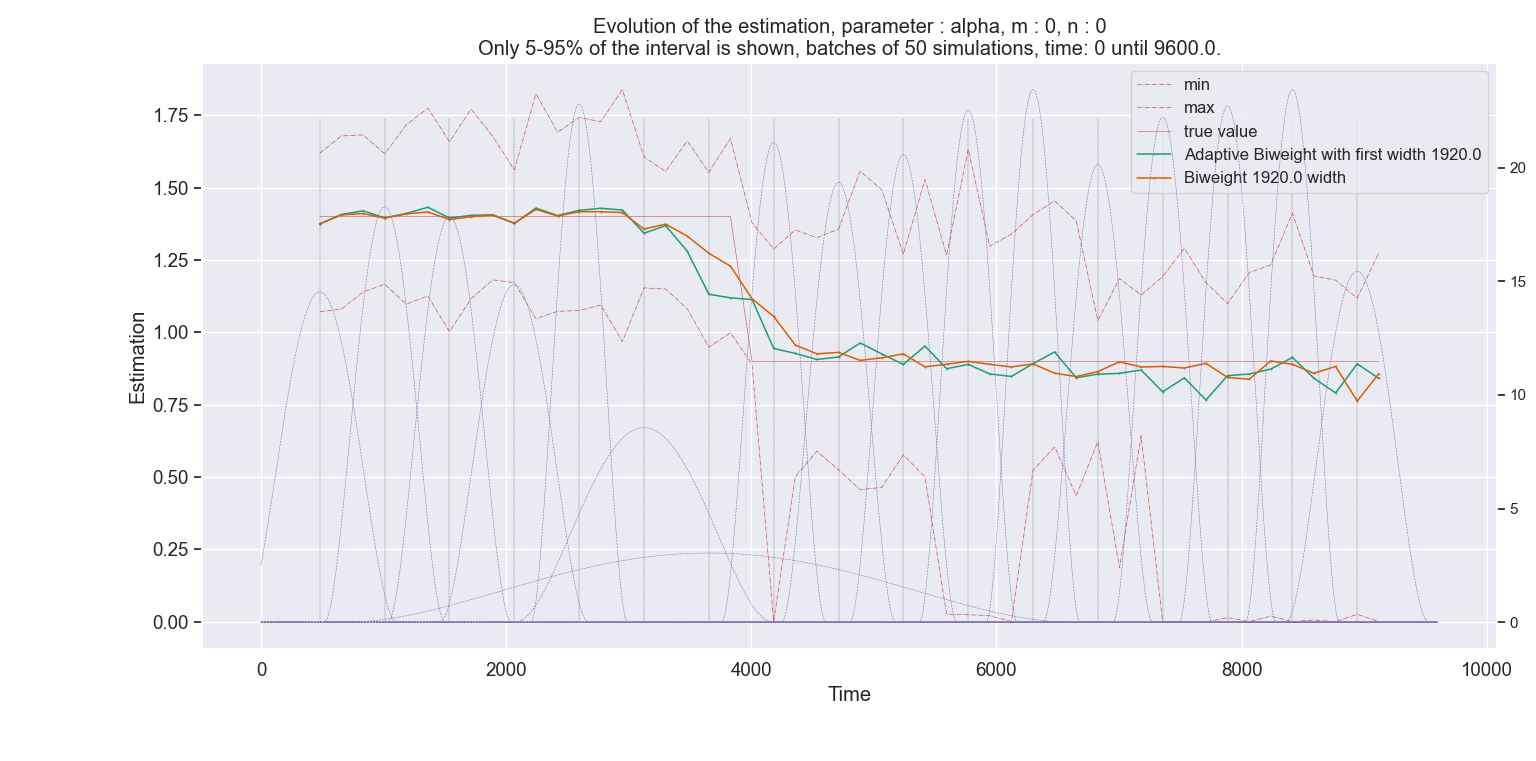
\includegraphics[width = 0.90 \textwidth]{../imag/chap3/2_bis/P.png}
\caption{TO WRITE.}
\label{fig:second_estimate_2_alpha}
\end{figure}

\begin{figure}
\centering
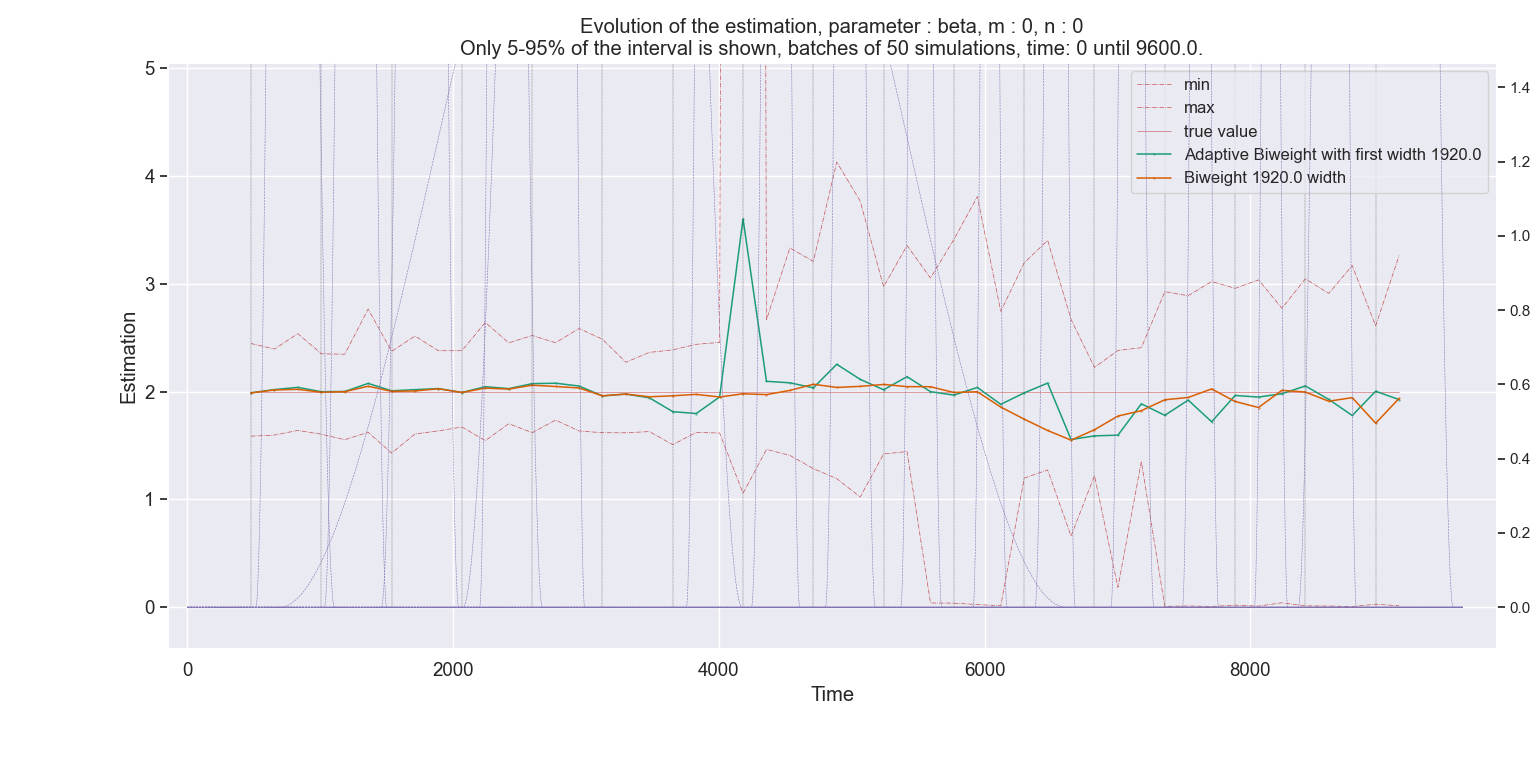
\includegraphics[width = 0.90 \textwidth]{../imag/chap3/2_bis/Q.png}
\caption{TO WRITE.}
\label{fig:second_estimate_2_beta}
\end{figure}

\begin{figure}
\centering
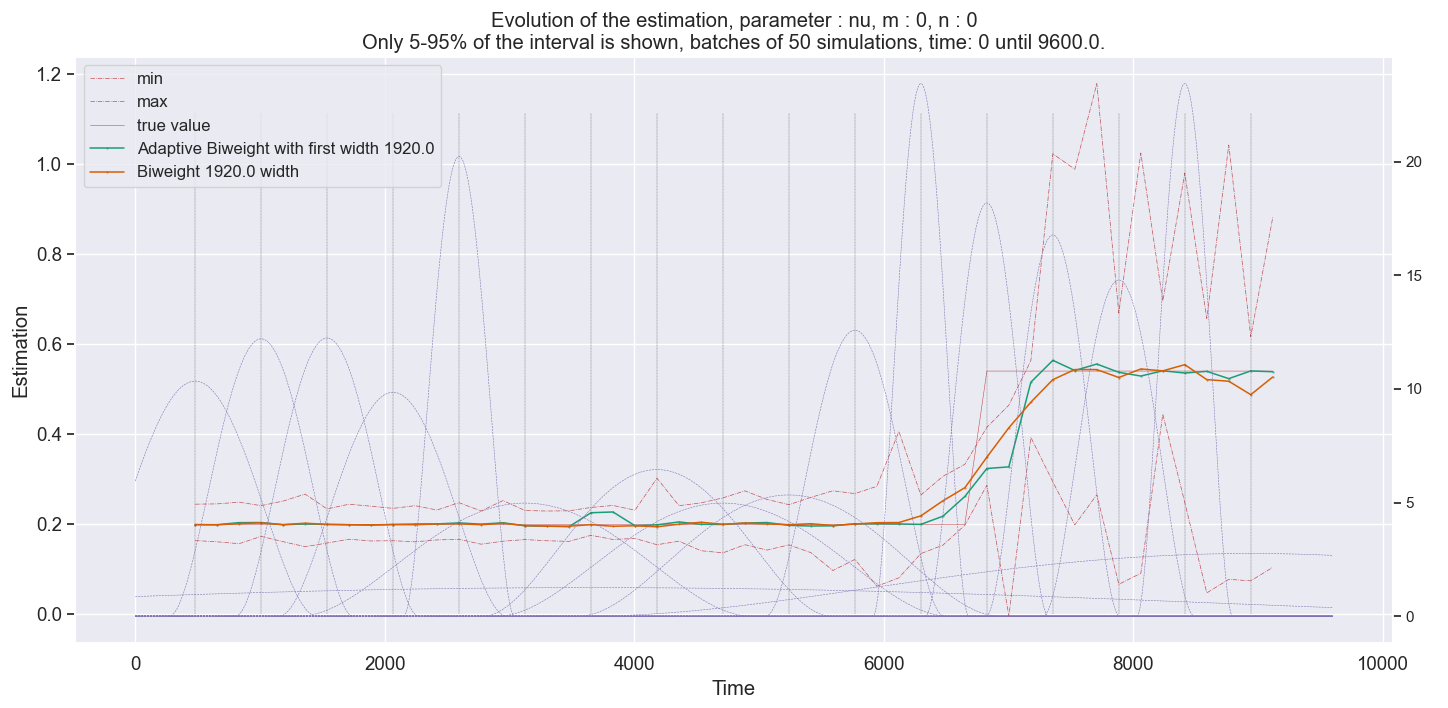
\includegraphics[width = 0.90 \textwidth]{../imag/chap3/2_bis/R.png}
\caption{TO WRITE.}
\label{fig:second_estimate_2_nu}
\end{figure}






\begin{figure}
\centering
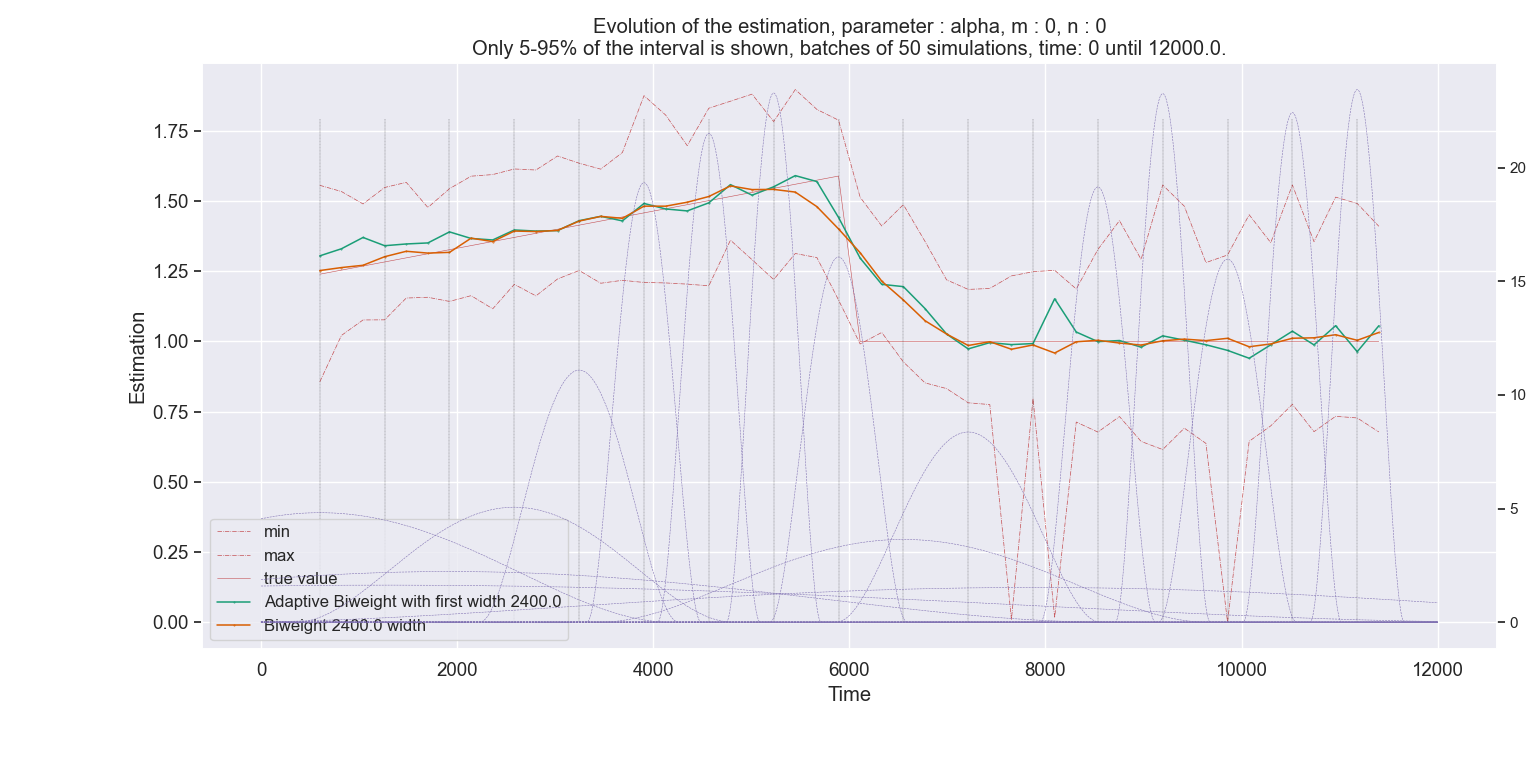
\includegraphics[width = 0.90 \textwidth]{../imag/chap3/3_bis/P.png}
\caption{TO WRITE.}
\label{fig:second_estimate_3_alpha}
\end{figure}

\begin{figure}
\centering
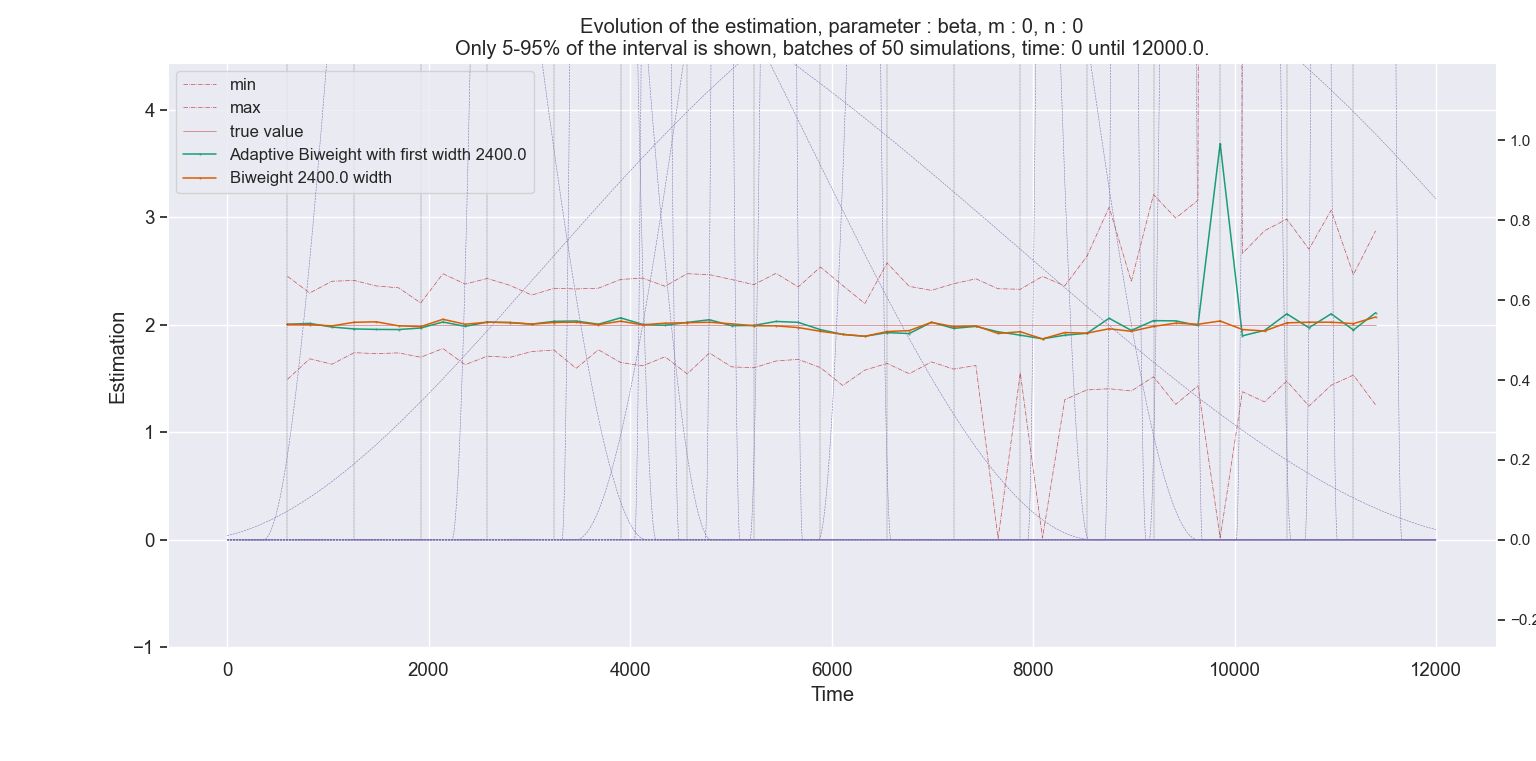
\includegraphics[width = 0.90 \textwidth]{../imag/chap3/3_bis/Q.png}
\caption{TO WRITE.}
\label{fig:second_estimate_3_beta}
\end{figure}

\begin{figure}
\centering
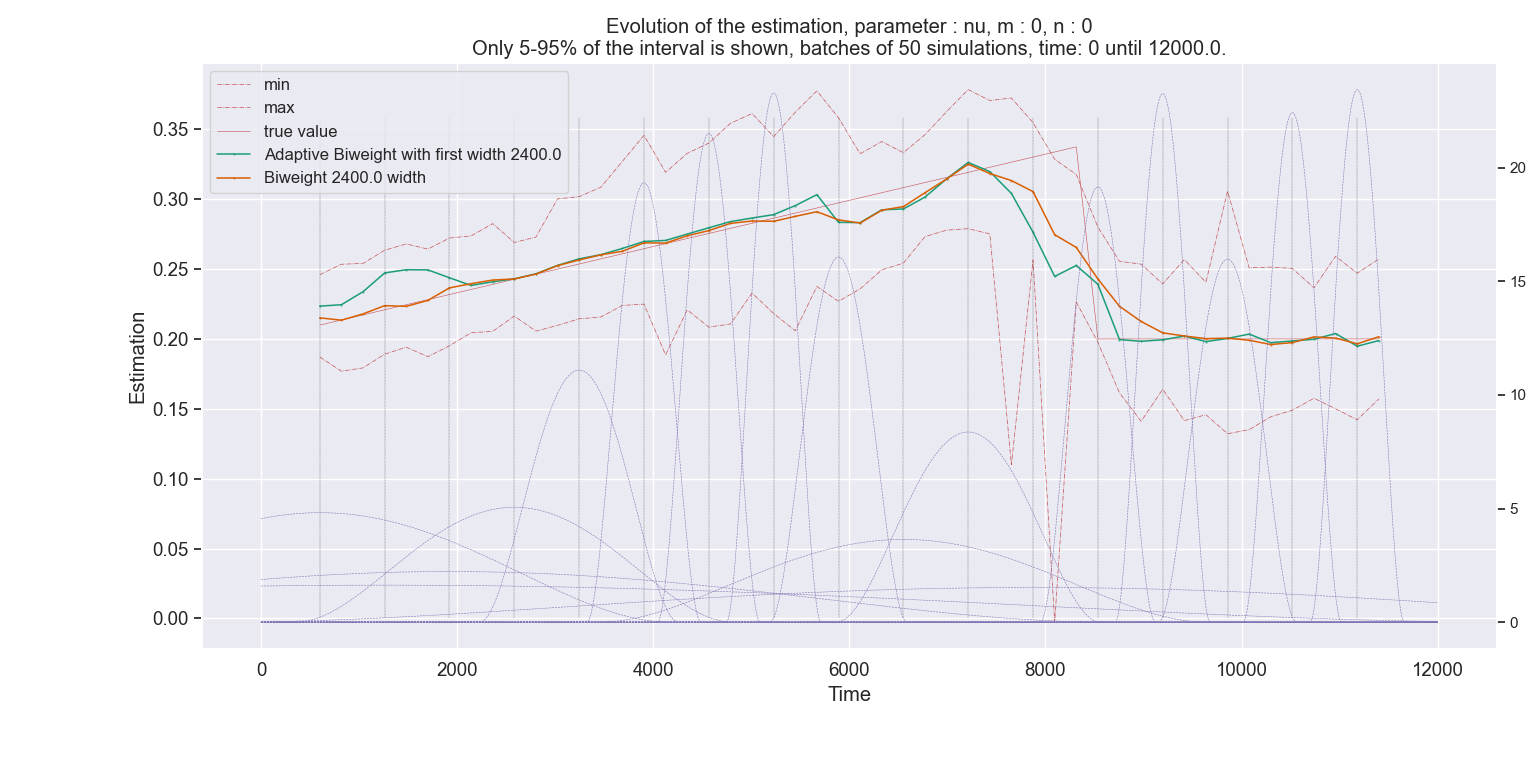
\includegraphics[width = 0.90 \textwidth]{../imag/chap3/3_bis/R.png}
\caption{TO WRITE.}
\label{fig:second_estimate_3_nu}
\end{figure}




\begin{figure}
\centering
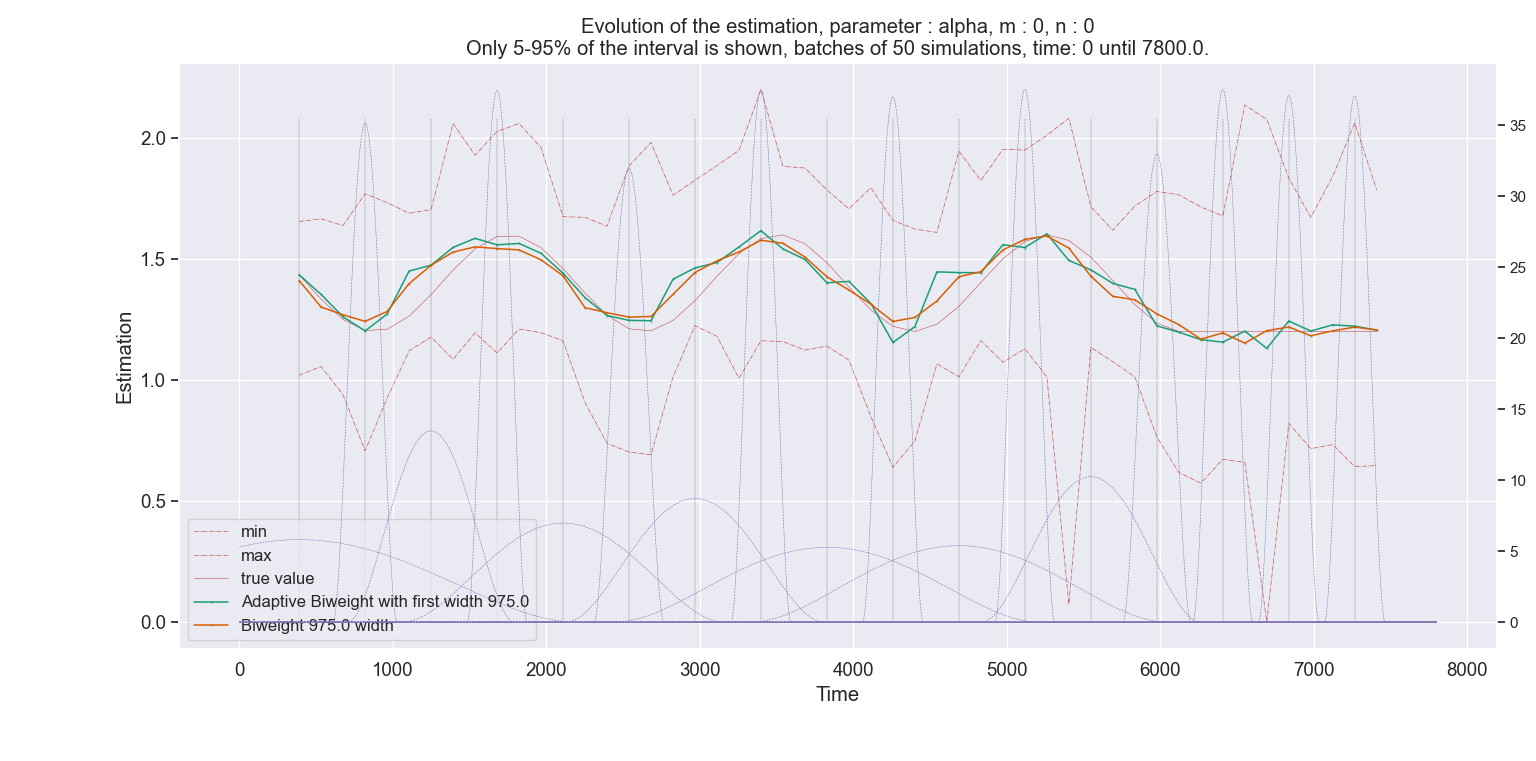
\includegraphics[width = 0.90 \textwidth]{../imag/chap3/4_bis/P.png}
\caption{TO WRITE.}
\label{fig:second_estimate_4_alpha}
\end{figure}

\begin{figure}
\centering
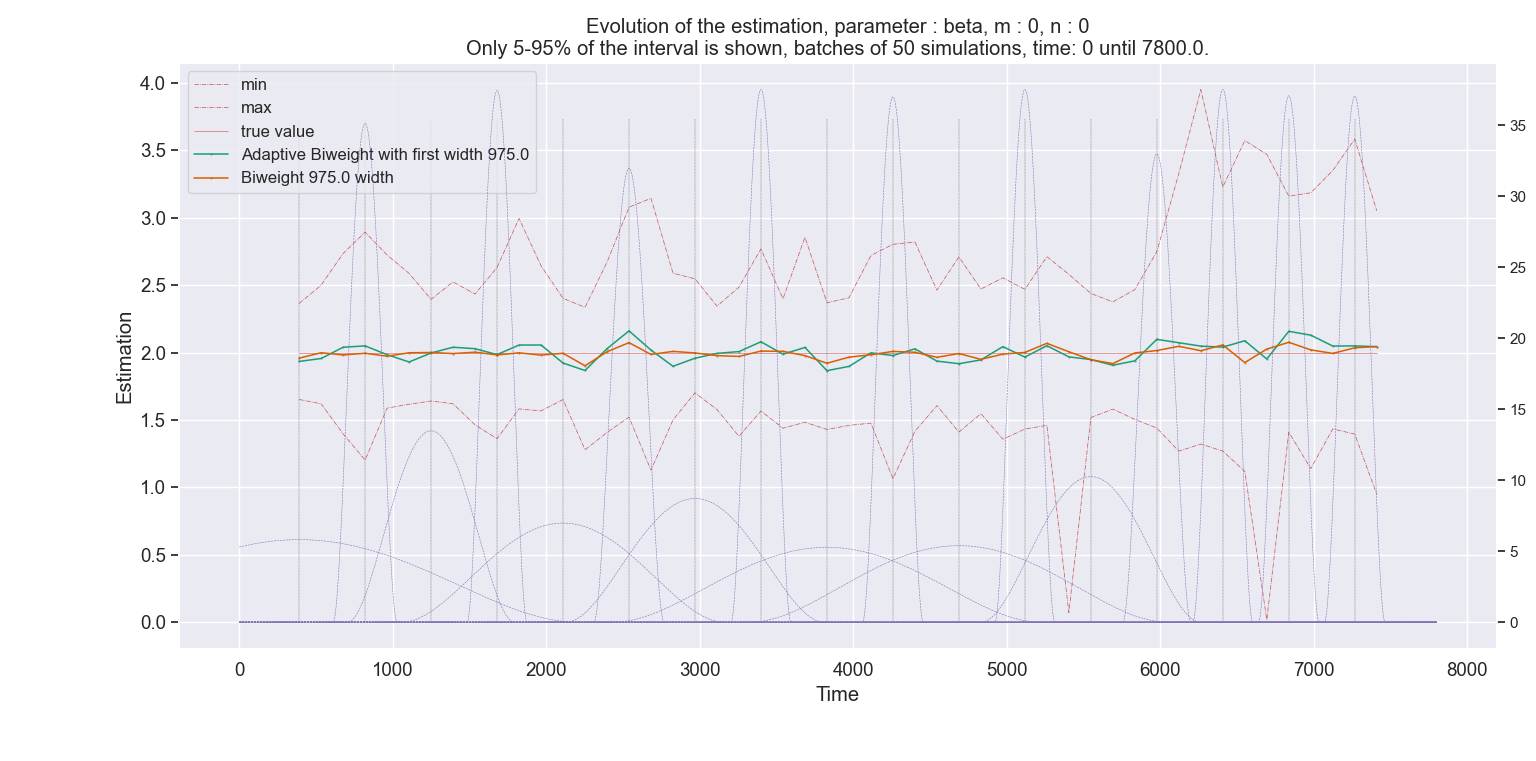
\includegraphics[width = 0.90 \textwidth]{../imag/chap3/4_bis/Q.png}
\caption{TO WRITE.}
\label{fig:second_estimate_4_beta}
\end{figure}

\begin{figure}
\centering
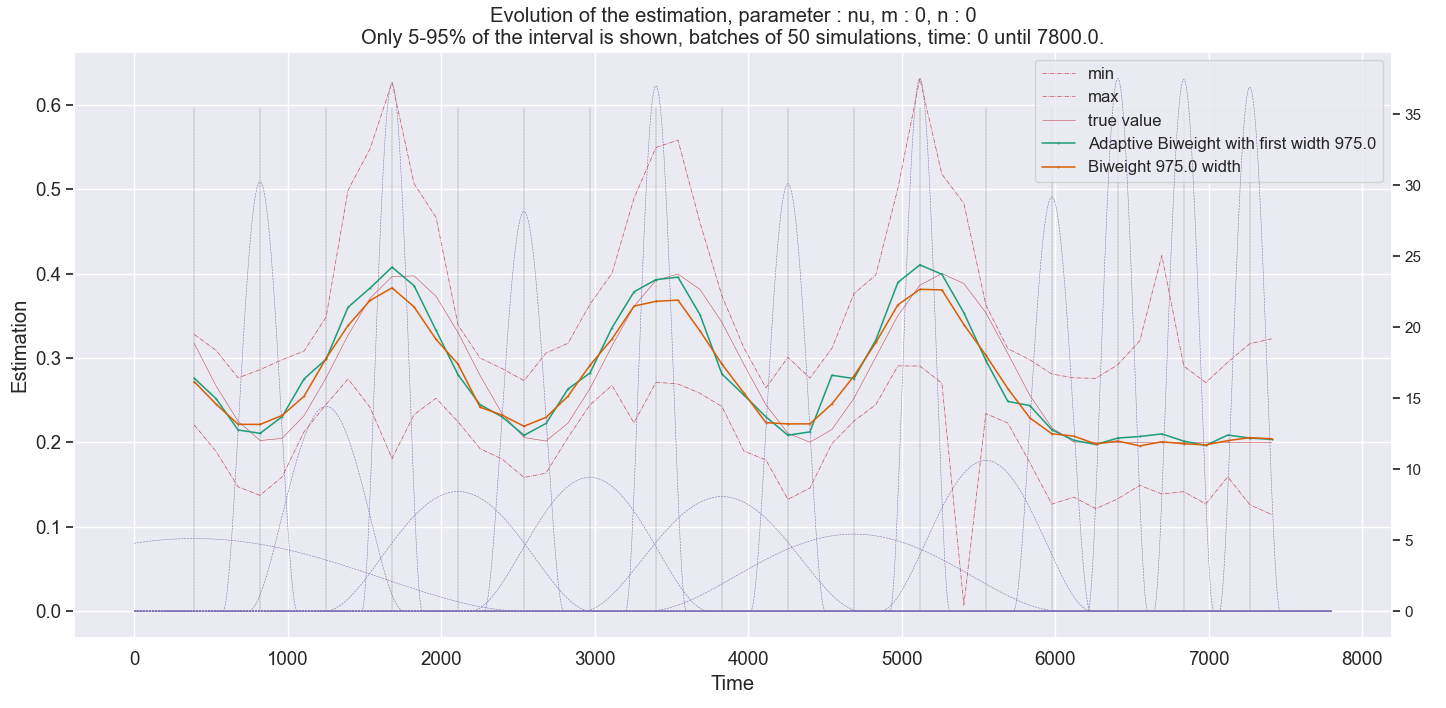
\includegraphics[width = 0.90 \textwidth]{../imag/chap3/4_bis/R.png}
\caption{TO WRITE.}
\label{fig:second_estimate_4_nu}
\end{figure}









